\section*{맥OS용 가상 머신 UTM 설정하기}
\addcontentsline{toc}{section}{맥OS용 가상 머신 UTM 설정하기} % 부록의 섹션도 목차에 추가
여러분이 맥북을 소유하고 있으며, 맥북에 가상머신을 설치하여 실습을 하고 싶다면 UTM을 사용하세요. 애플 실리콘이 장착된 맥북에서는 버추얼 박스를 사용하지 못합니다. UTM은 iOS나 맥OS 에서 실행되는 가상 머신입니다. UTM을 사용하면 맥OS 기기에서 Linux, Windows, FreeBSD, Solaris, Haiku OS 등을 실행할 수 있습니다. UTM을 사용하면 iOS 기기에서 Docker를 실행할 수 있습니다. 

UTM은 항상 완전히 무료이고 오픈 소스입니다. Mac App Store 버전은 GitHub 버전과 동일하며, 누락된 기능은 없습니다. Mac App Store 버전의 유일한 이점은 자동 업데이트를 받을 수 있다는 것입니다. App Store 버전을 구매하면 UTM 개발에 직접적인 자금을 제공하며, 당신의 지지를 표현할 수 있습니다.

UTM을 사용하려면 다음 단계를 따르세요:
\begin{enumerate}
    \item UTM 앱을 다운로드하고 설치하세요. download from github(무료)를 선택하세요. \\$https://docs.getutm.app/installation/macos/$
    \item 우분투 20.04 LTS 이미지를 다운로드하세요. \\$https://ubuntu.com/download/desktop$
    \item UTM 앱을 실행하고, 아래 그림과 같이 "+" 버튼을 눌러 새 가상 머신을 추가하세요. (우분투 20.04 LTS를 선택하세요.)
    \item 가상 머신을 추가하면, 아래 그림과 같이 설정을 변경하세요.
    \item 가상 머신을 시작하고, 아래 그림과 같이 가상 머신에 접속하세요.
\end{enumerate}

\subsection{UTM을 이용하여 Ubuntu 설치하기}

\begin{figure}[htbp]
    \centering
    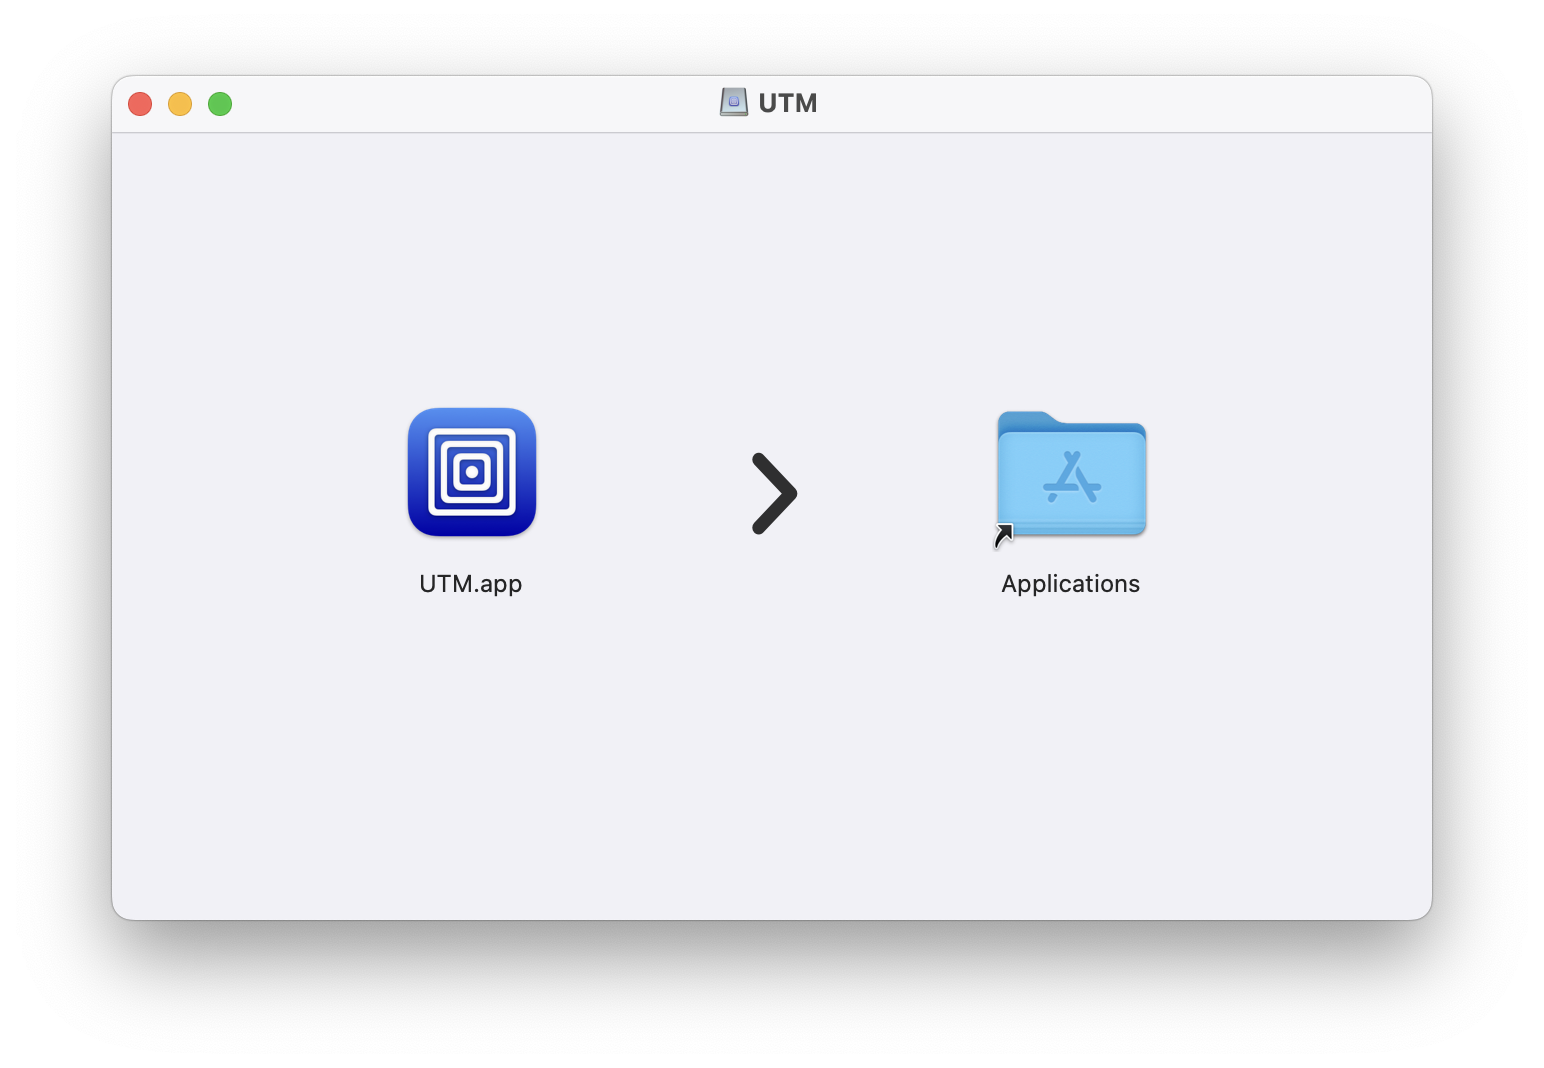
\includegraphics[width=0.9\textwidth]{images/chapter2Images/ch2_image_01.png}
    \caption{설치 프로세스 시작}
\end{figure}

\begin{figure}[htbp]
    \centering
    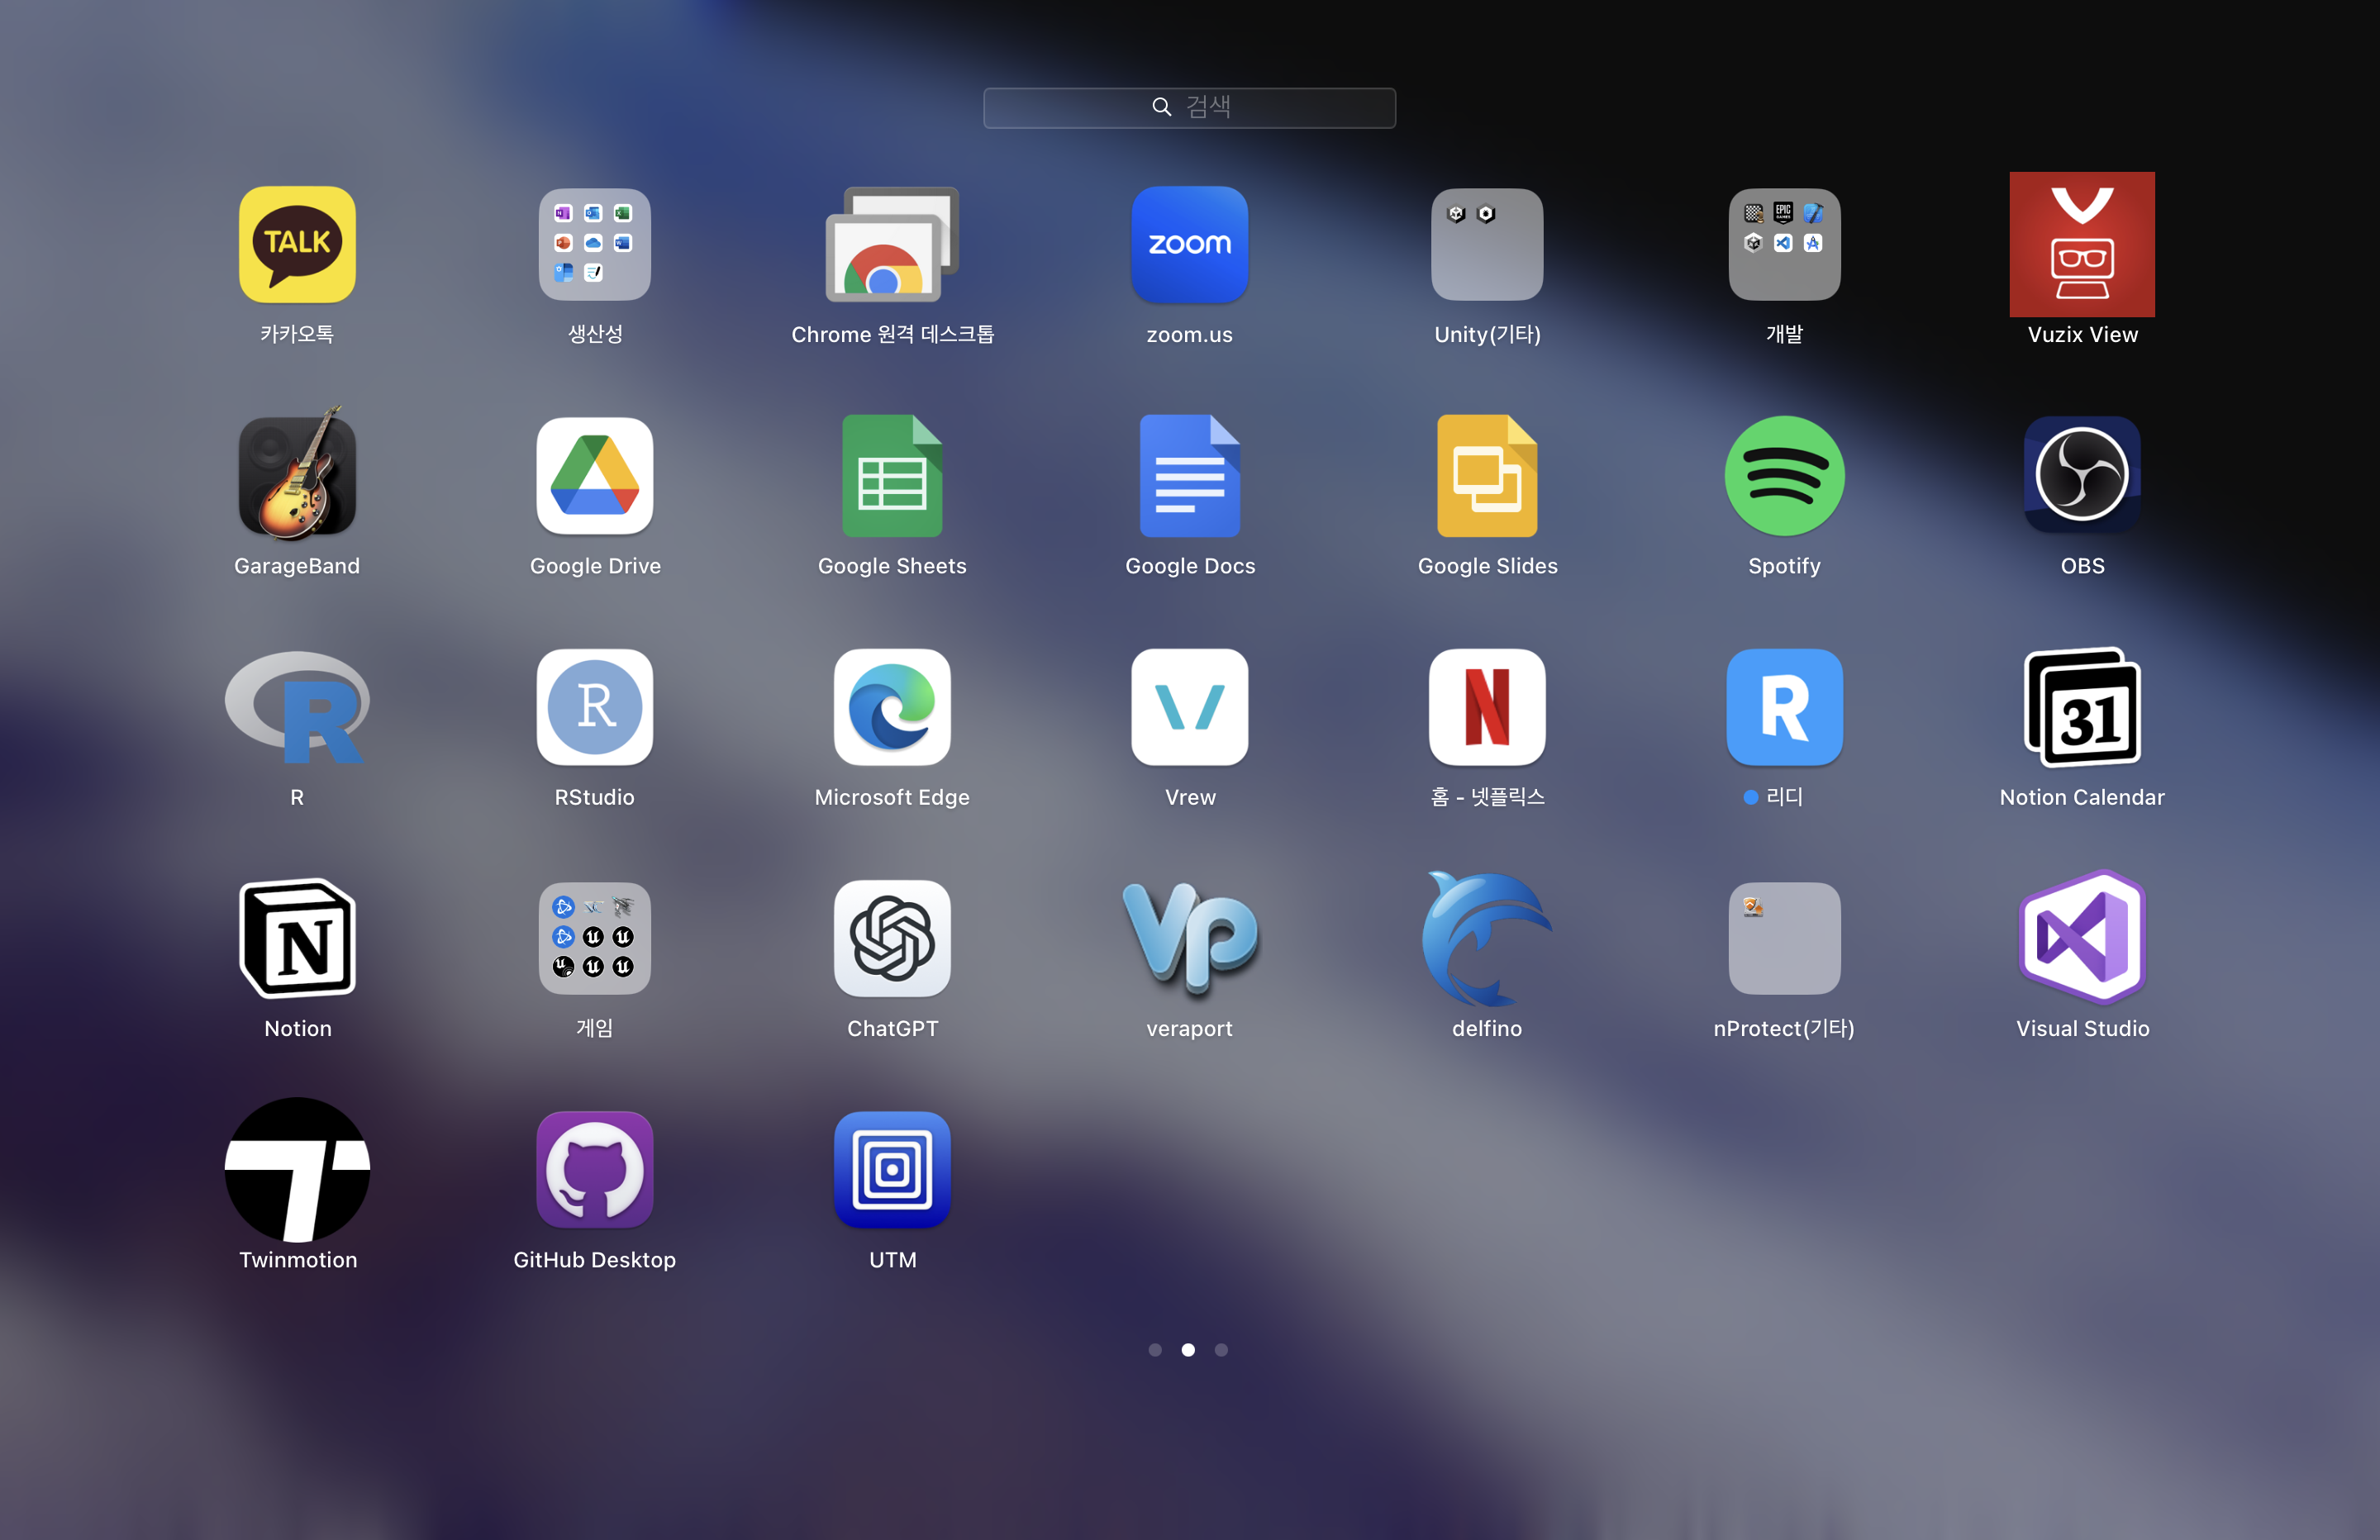
\includegraphics[width=0.9\textwidth]{images/chapter2Images/ch2_image_02.png}
    \caption{설치 언어 선택}
\end{figure}

\begin{figure}[htbp]
    \centering
    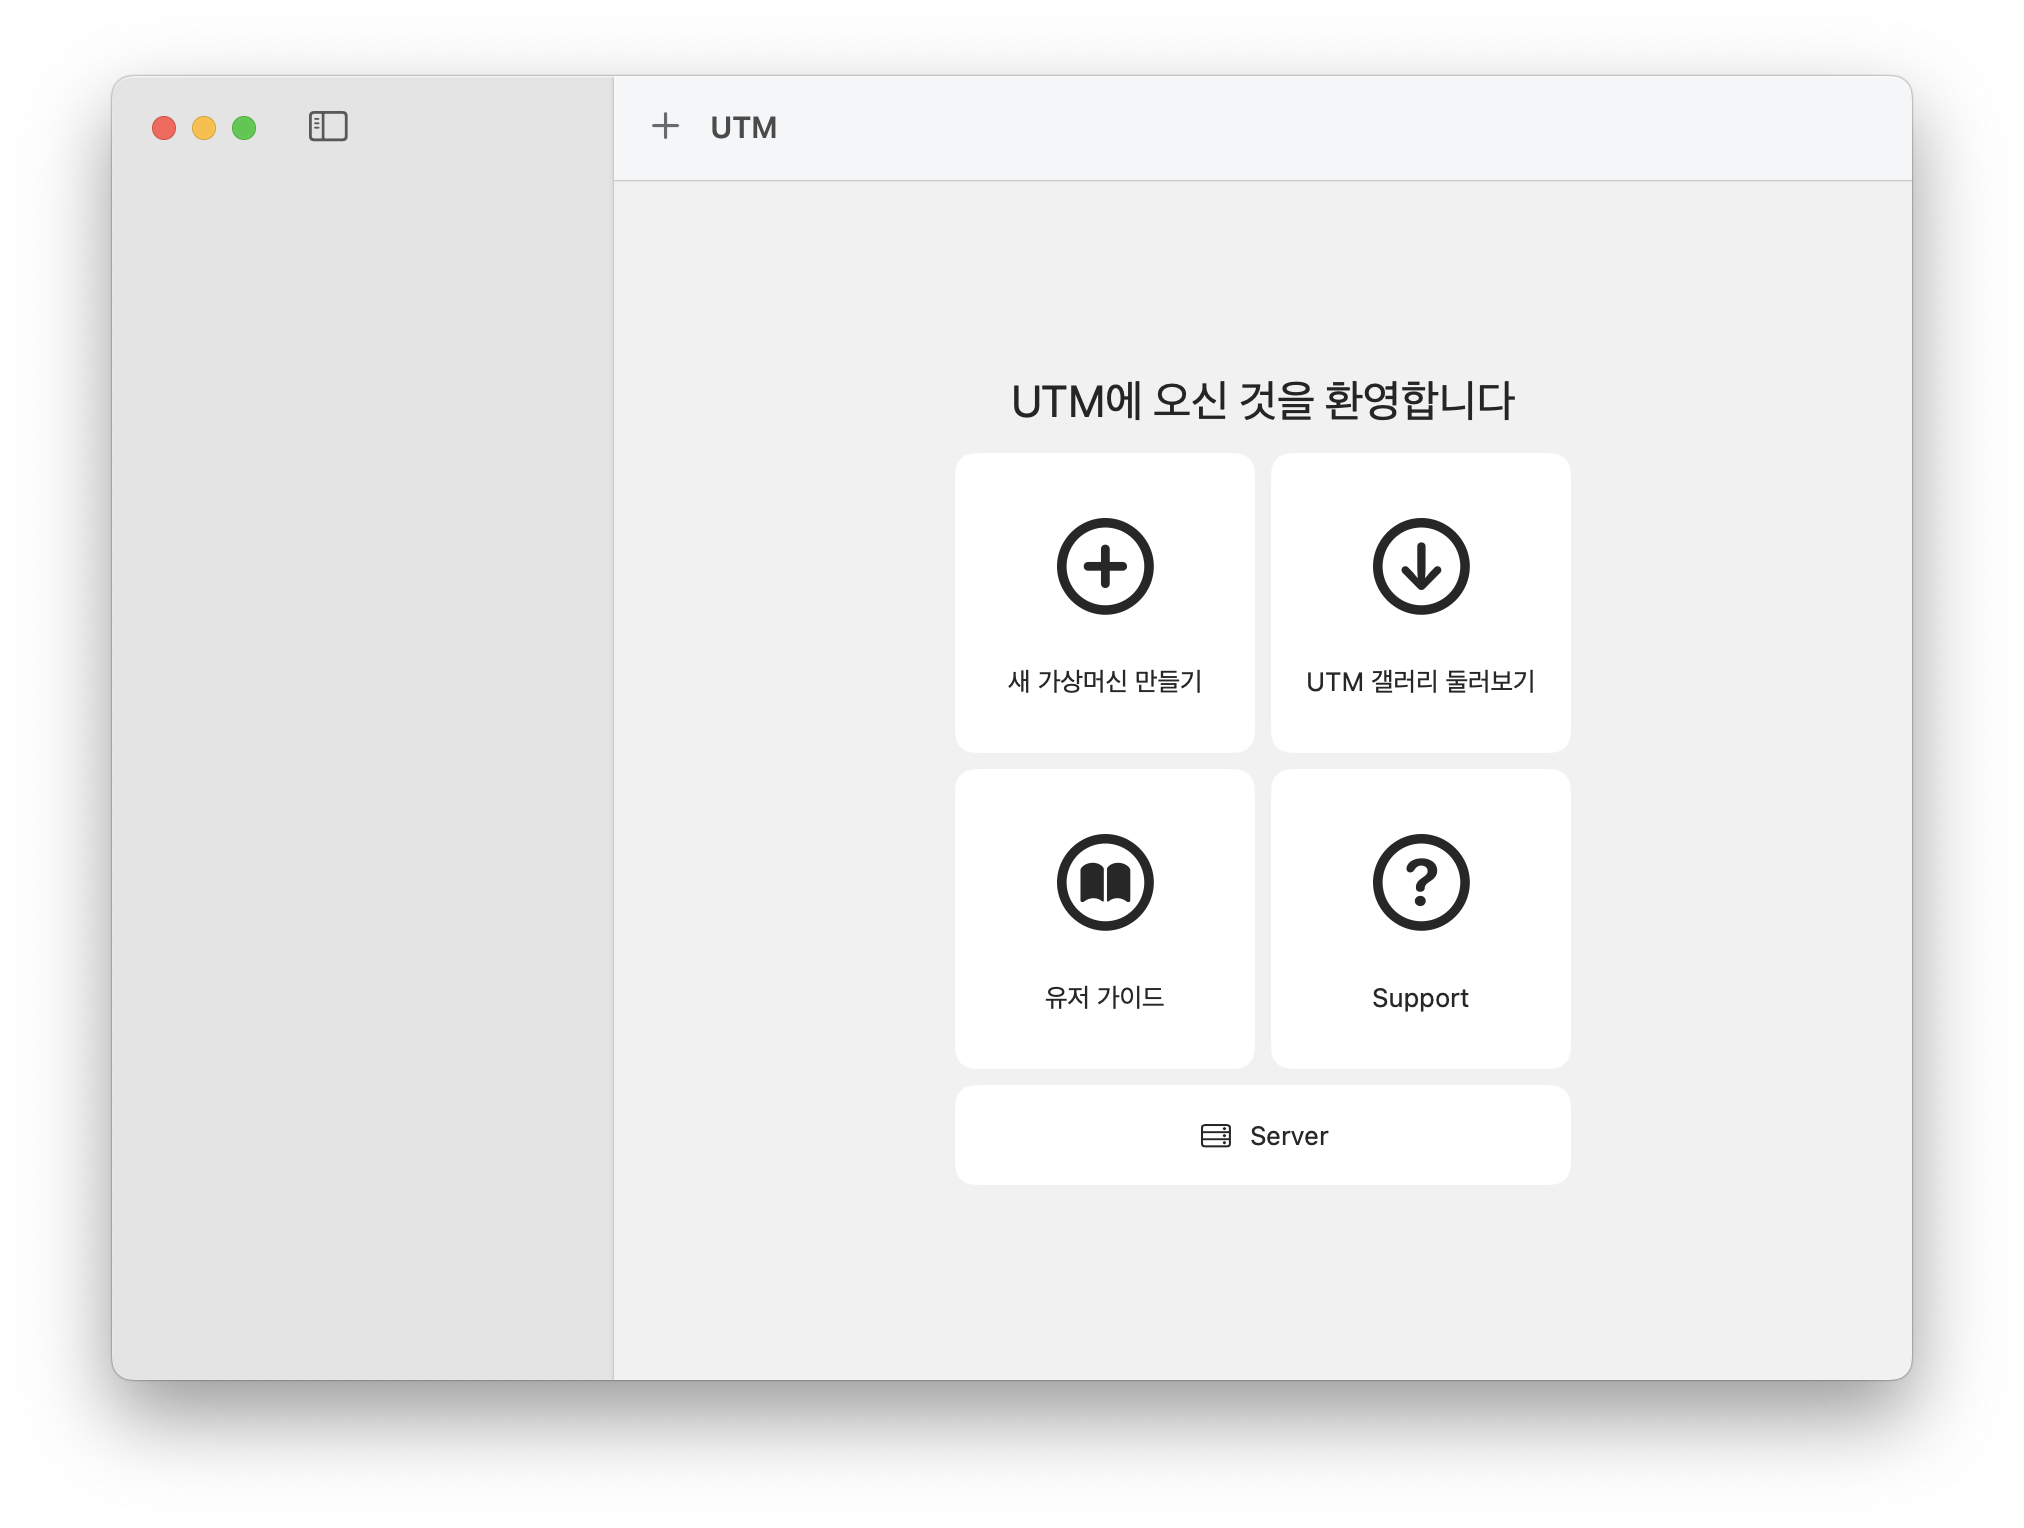
\includegraphics[width=0.9\textwidth]{images/chapter2Images/ch2_image_03.png}
    \caption{설치 준비}
\end{figure}

\begin{figure}[htbp]
    \centering
    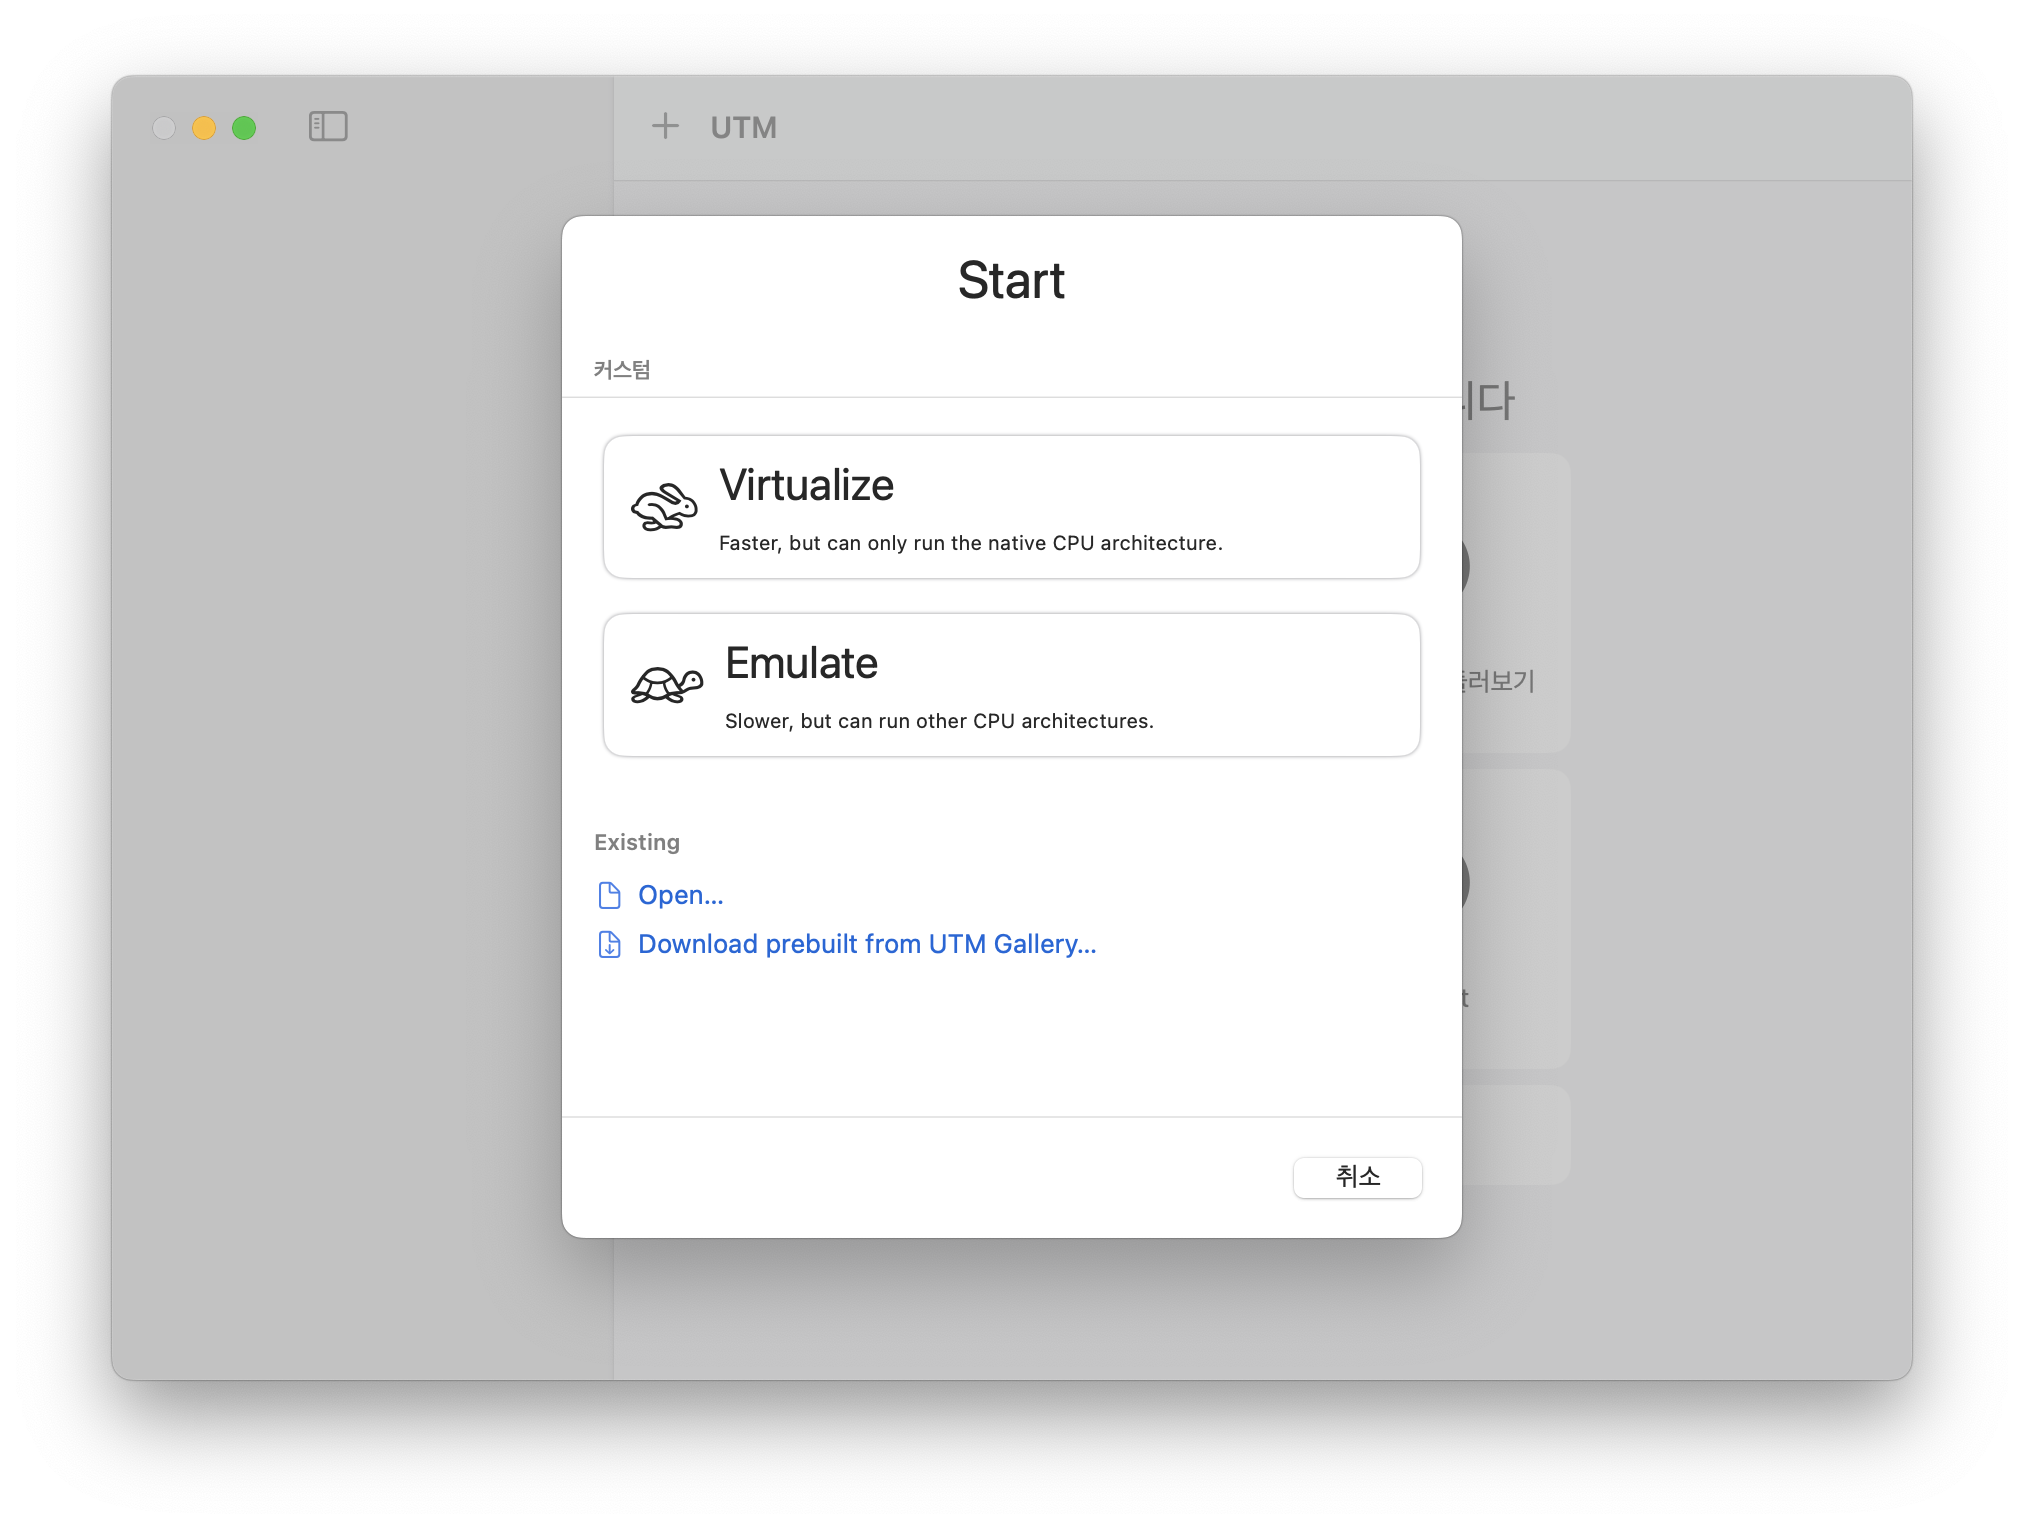
\includegraphics[width=0.9\textwidth]{images/chapter2Images/ch2_image_04.png}
    \caption{시스템 구성}
\end{figure}

\begin{figure}[htbp]
    \centering
    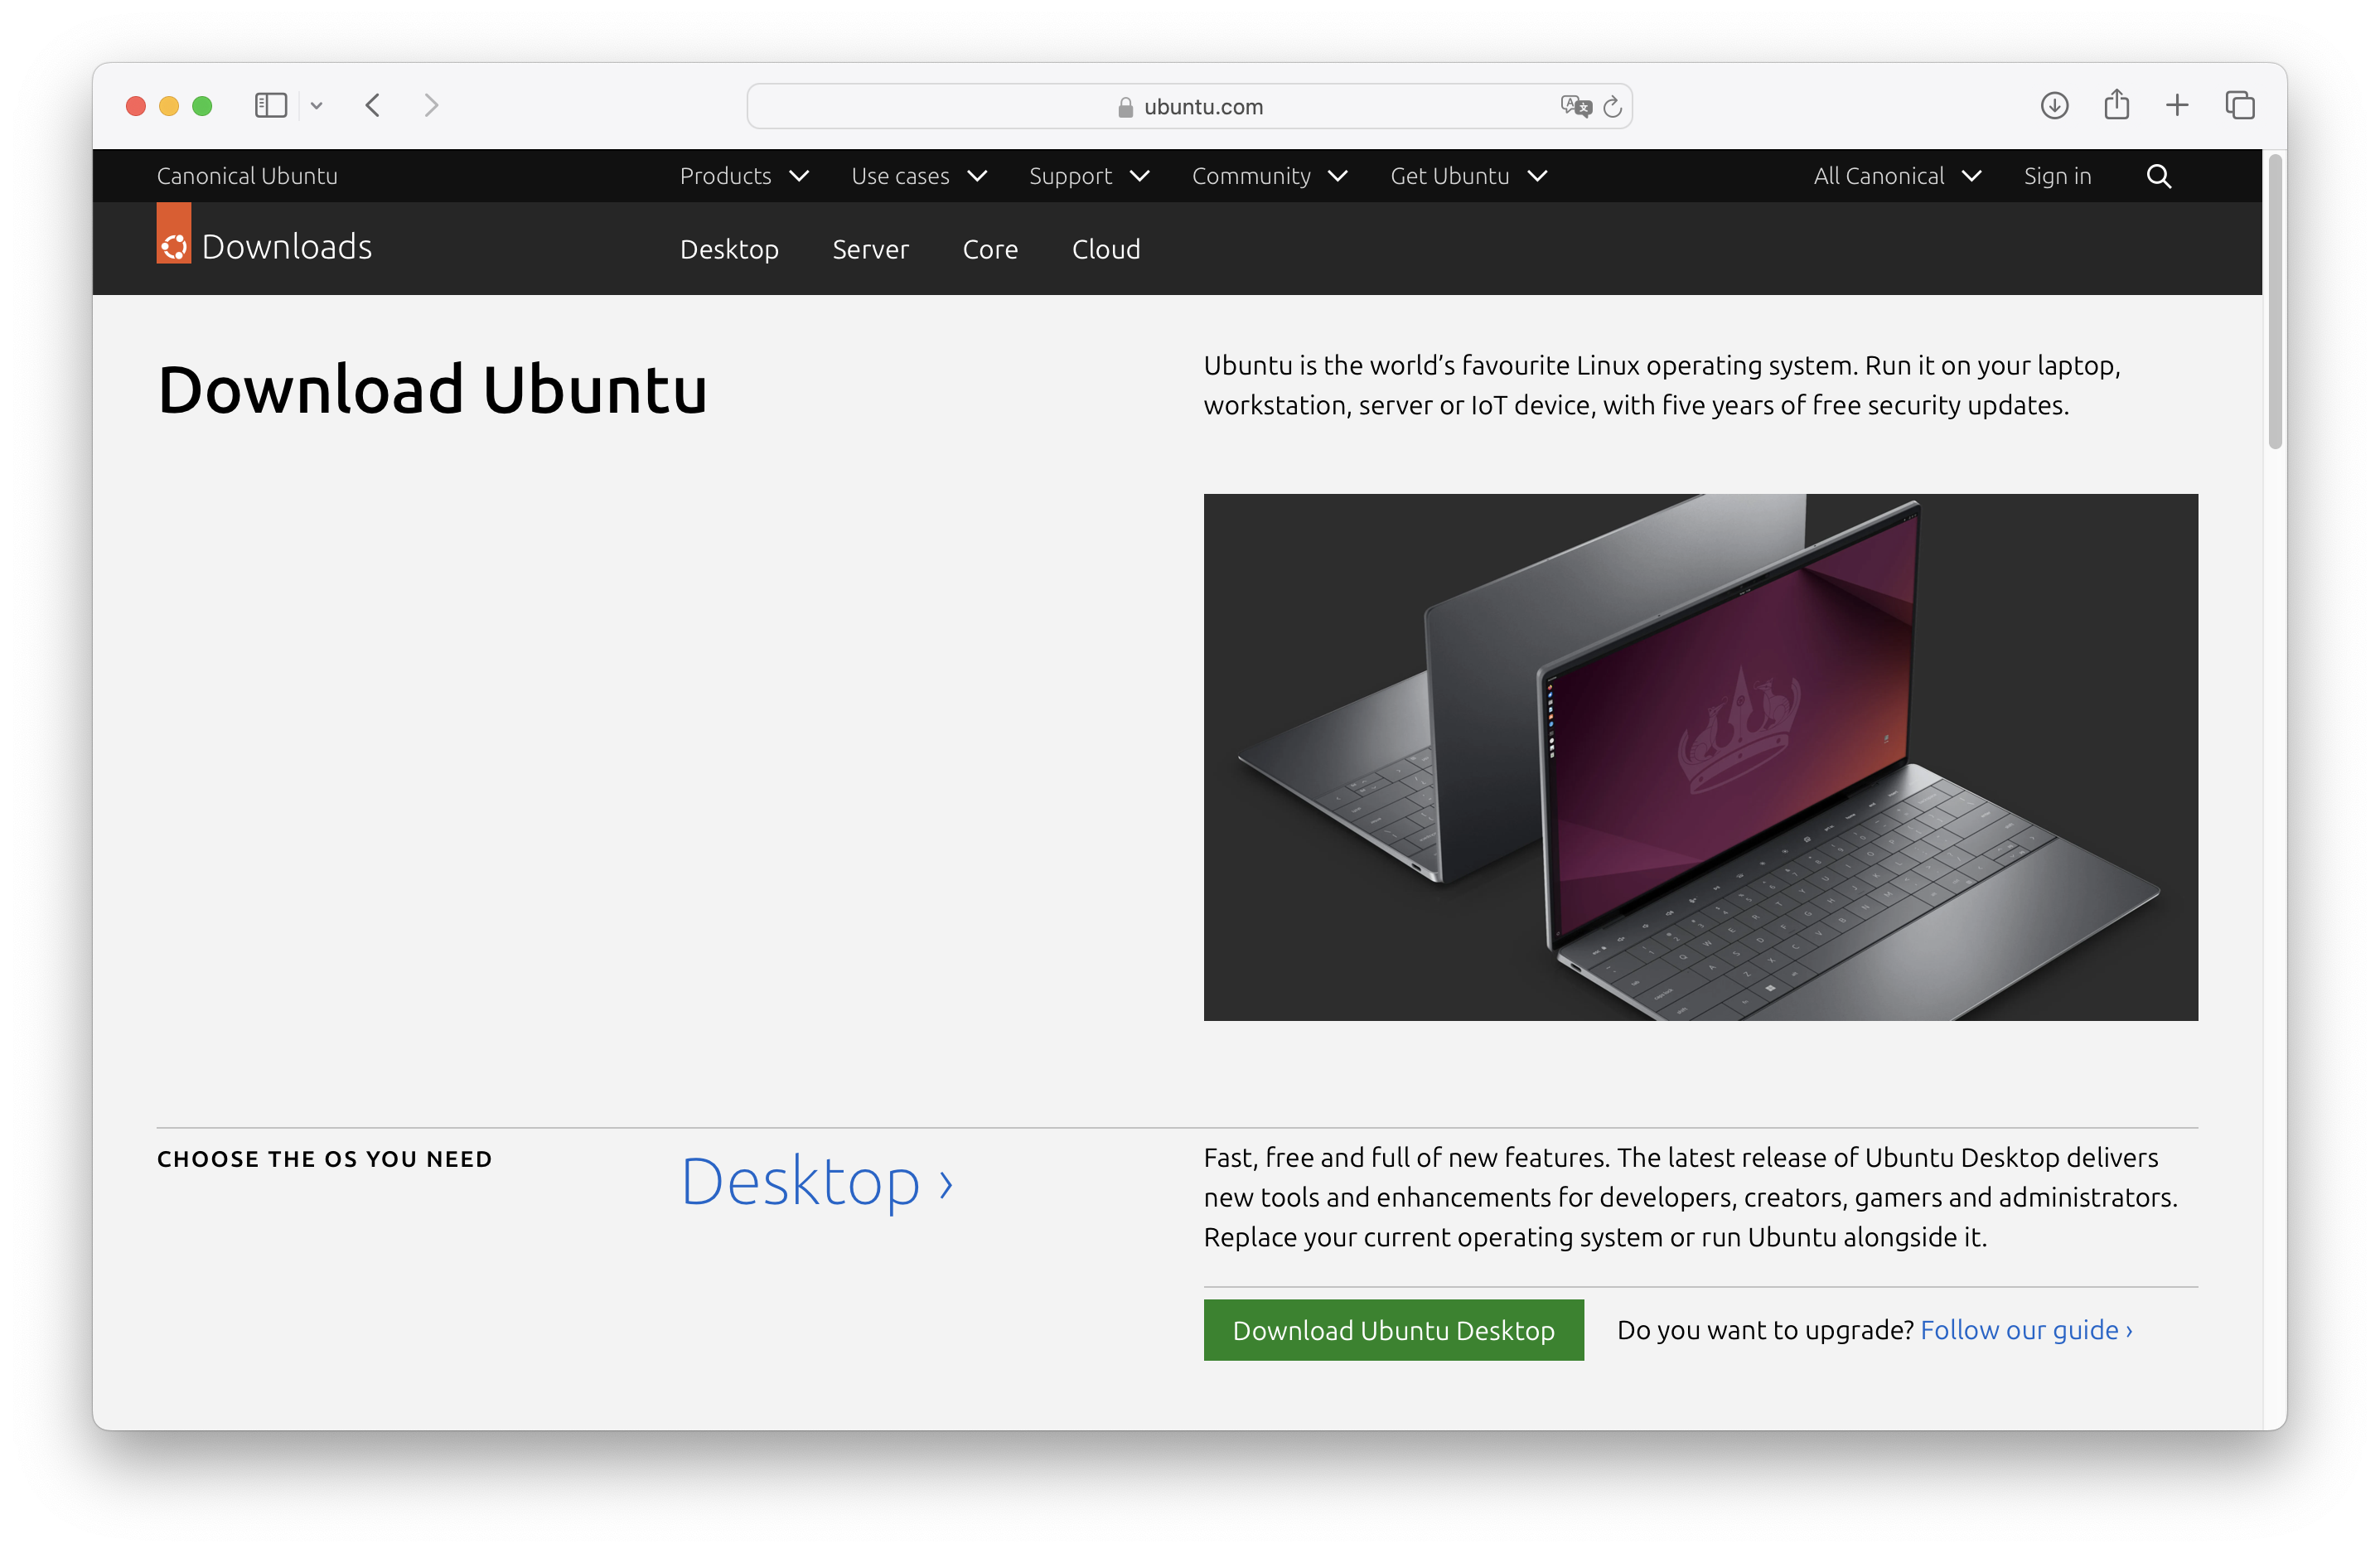
\includegraphics[width=0.9\textwidth]{images/chapter2Images/ch2_image_05.png}
    \caption{시스템 파일 설치}
\end{figure}

\begin{figure}[htbp]
    \centering
    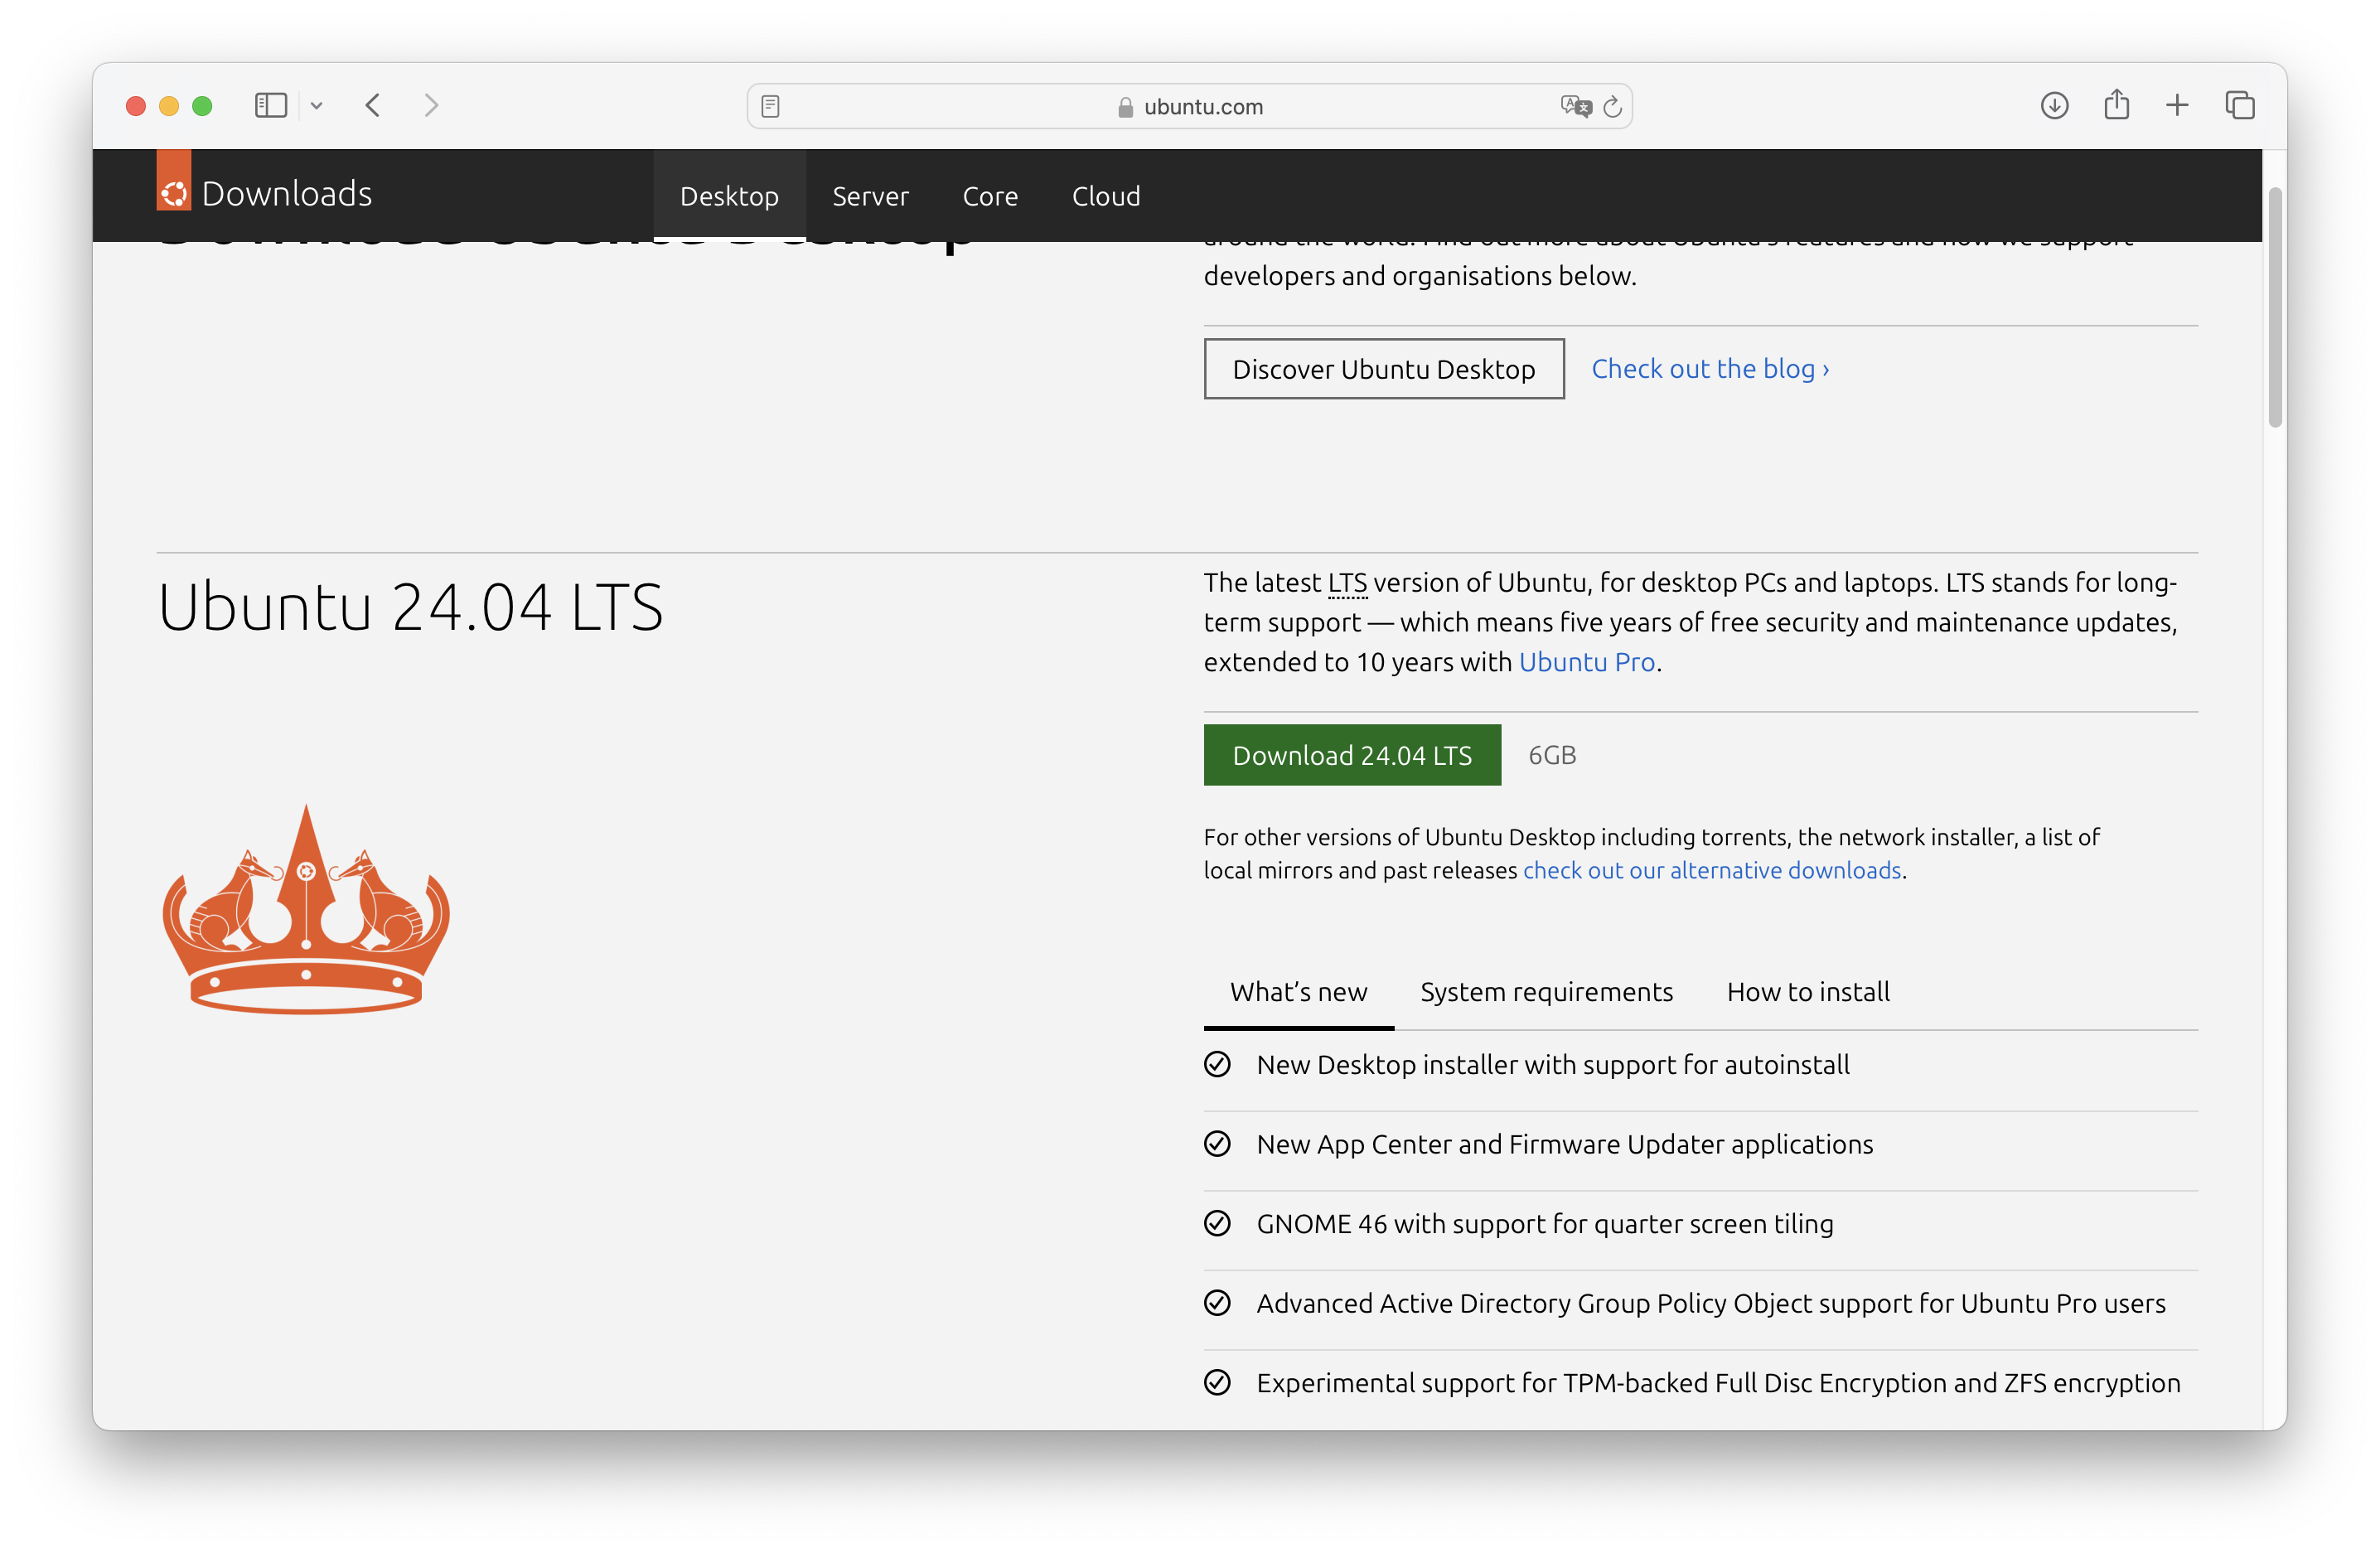
\includegraphics[width=0.9\textwidth]{images/chapter2Images/ch2_image_06.png}
    \caption{설치 완료}
\end{figure}

\begin{figure}[htbp]
    \centering
    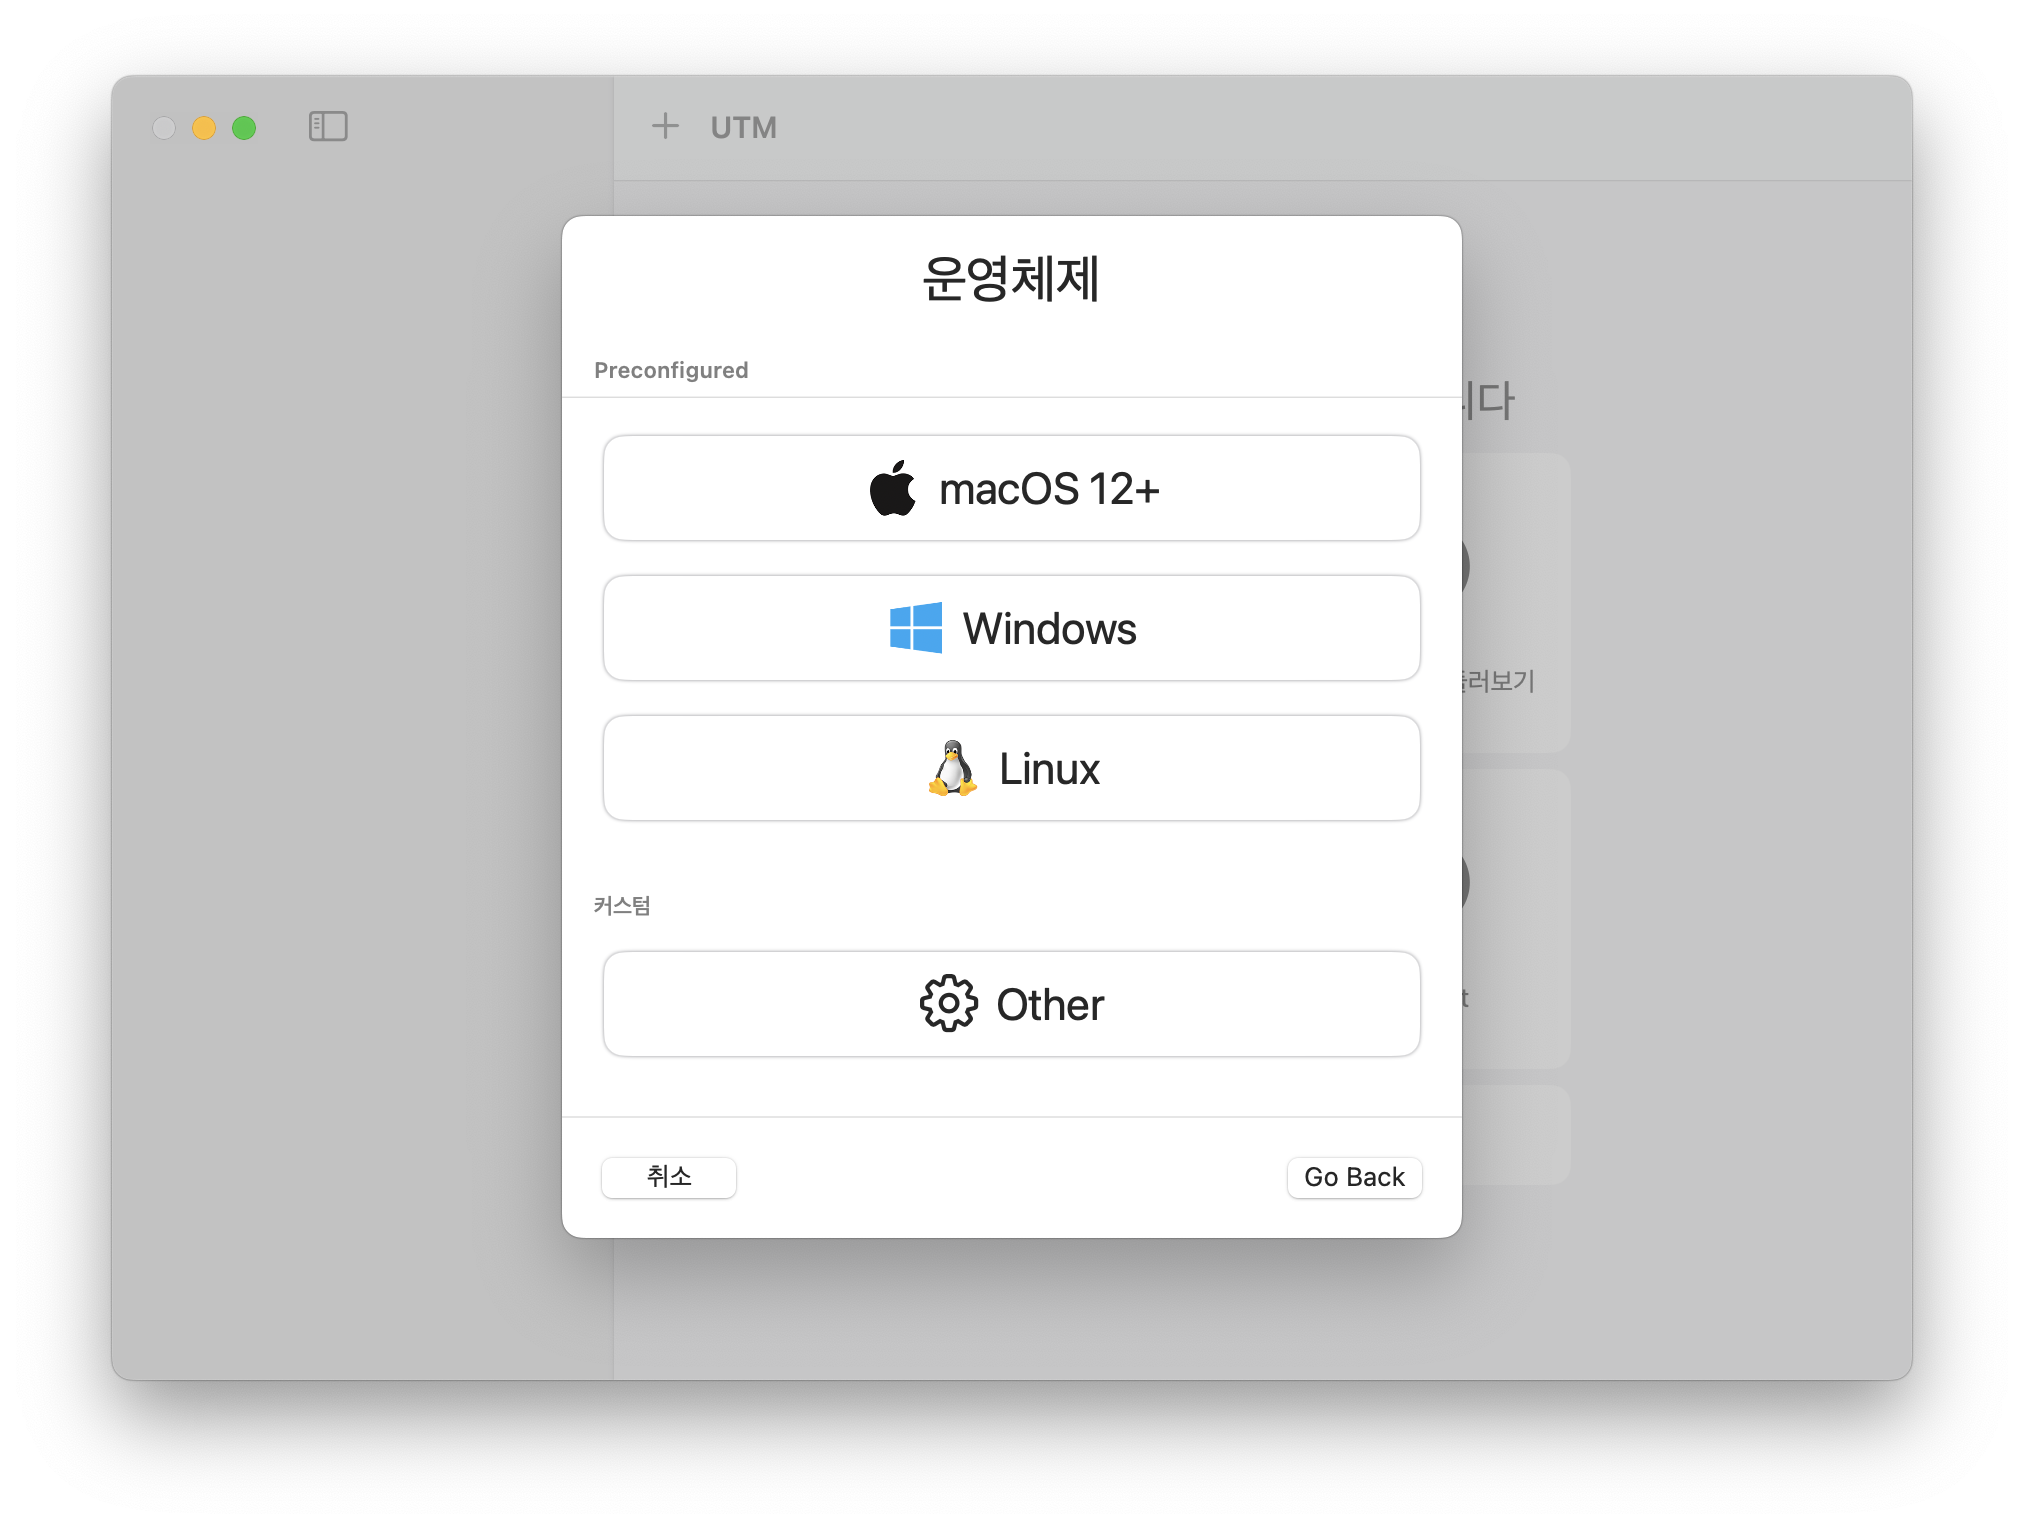
\includegraphics[width=0.9\textwidth]{images/chapter2Images/ch2_image_07.png}
    \caption{시스템 재시작}
\end{figure}

\begin{figure}[htbp]
    \centering
    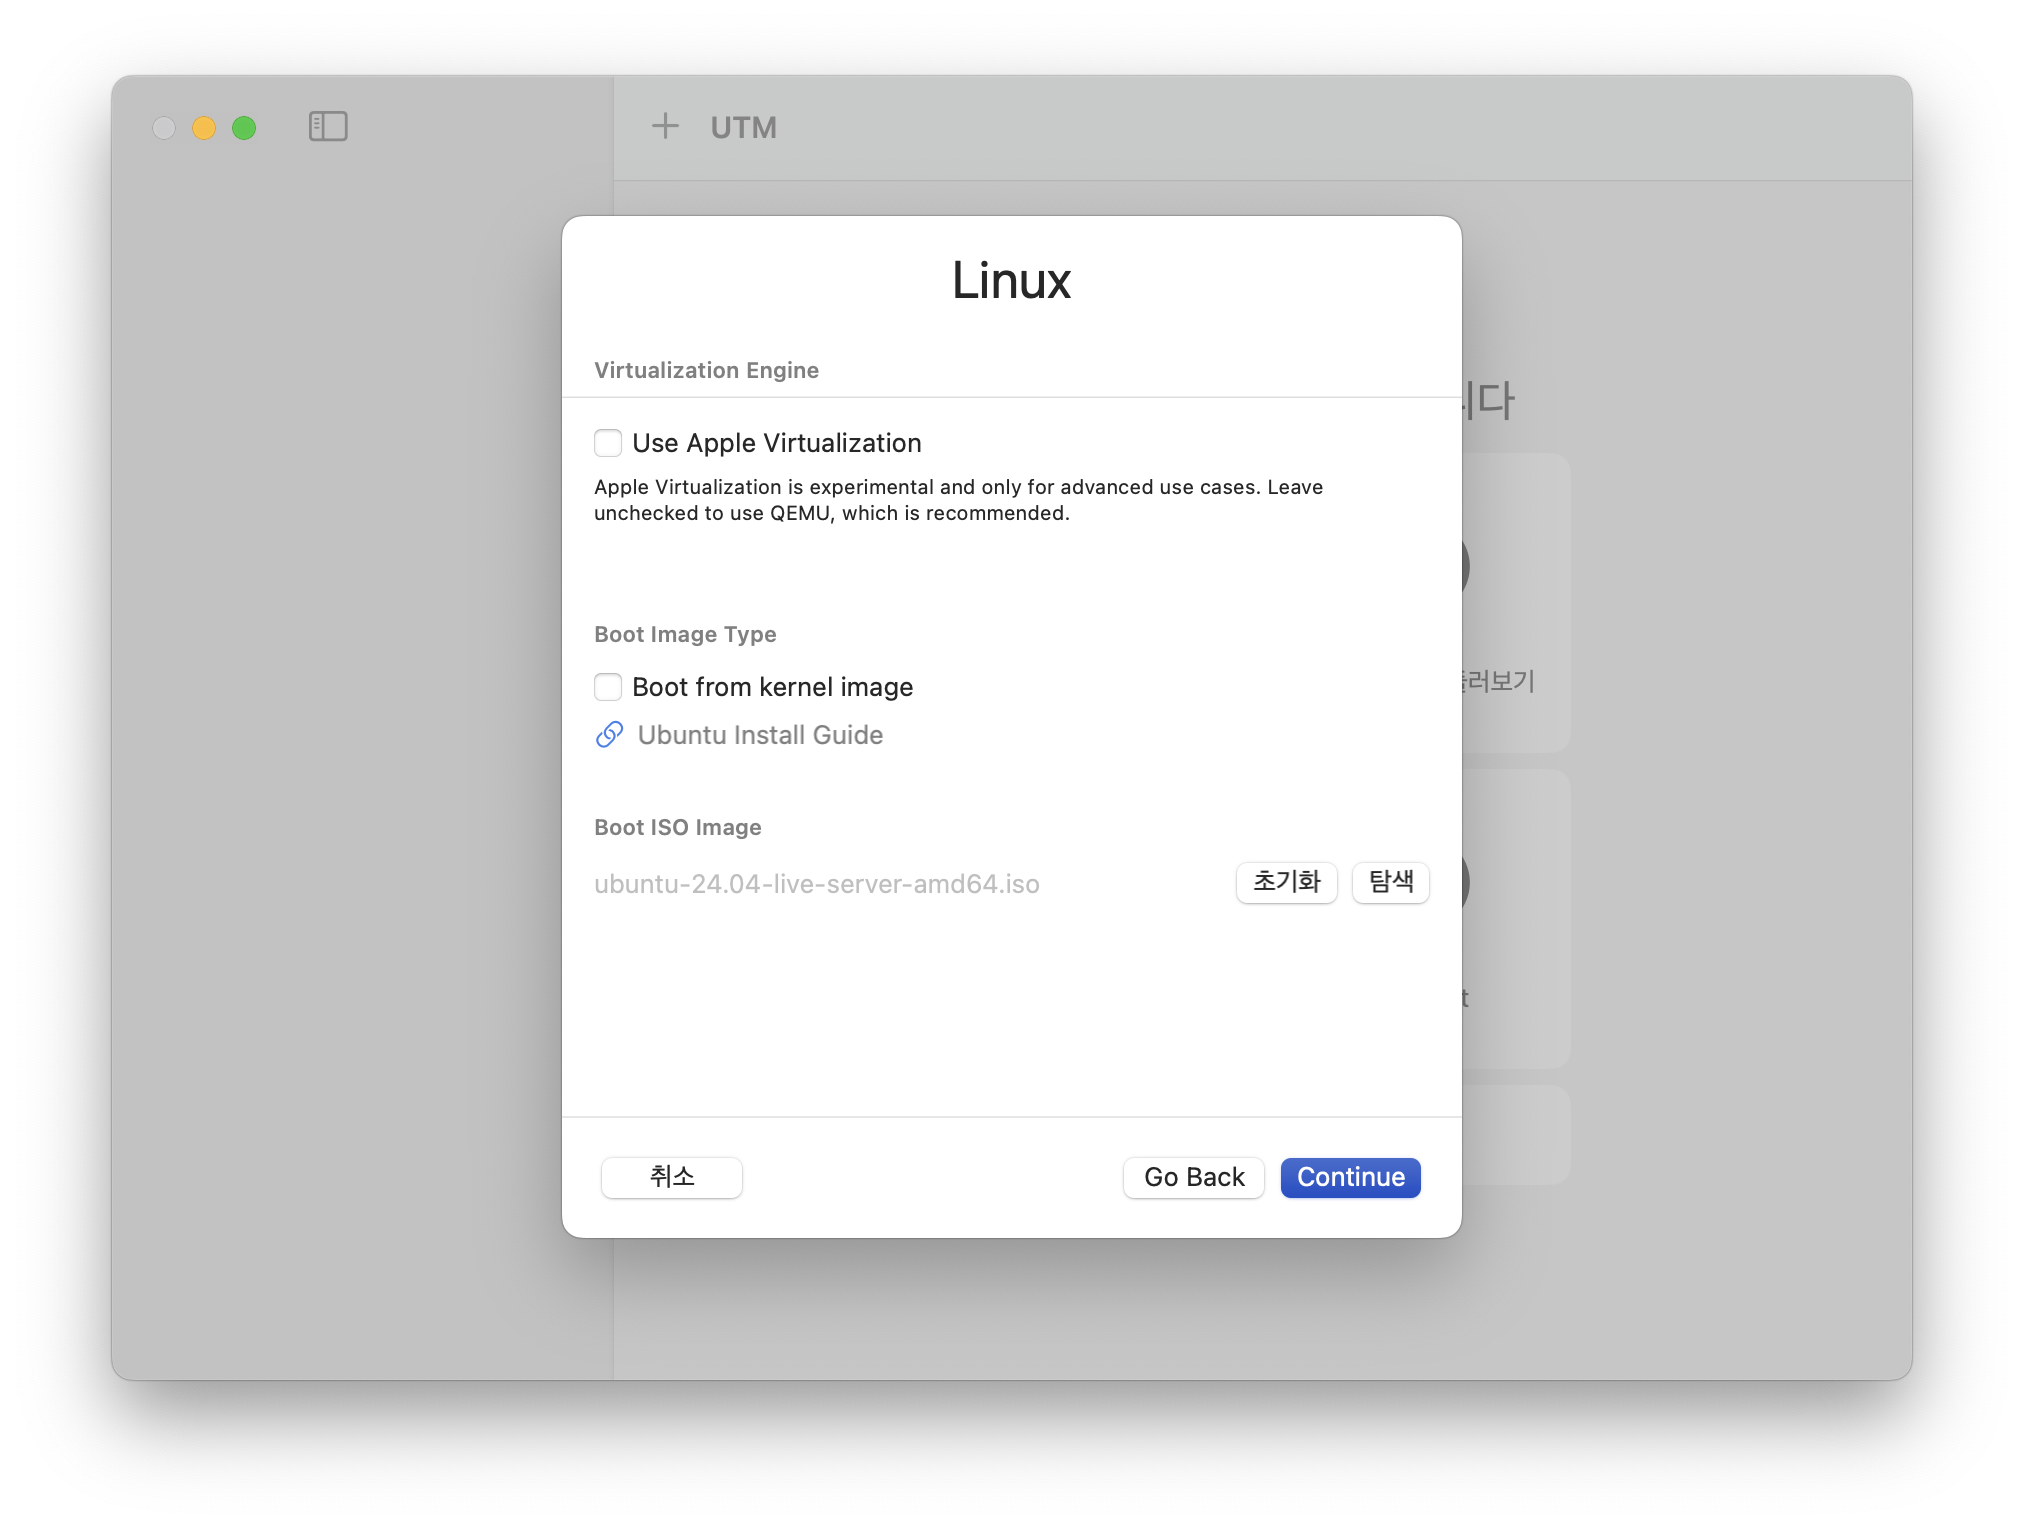
\includegraphics[width=0.9\textwidth]{images/chapter2Images/ch2_image_08.png}
    \caption{설정 완료}
\end{figure}

\begin{figure}[htbp]
    \centering
    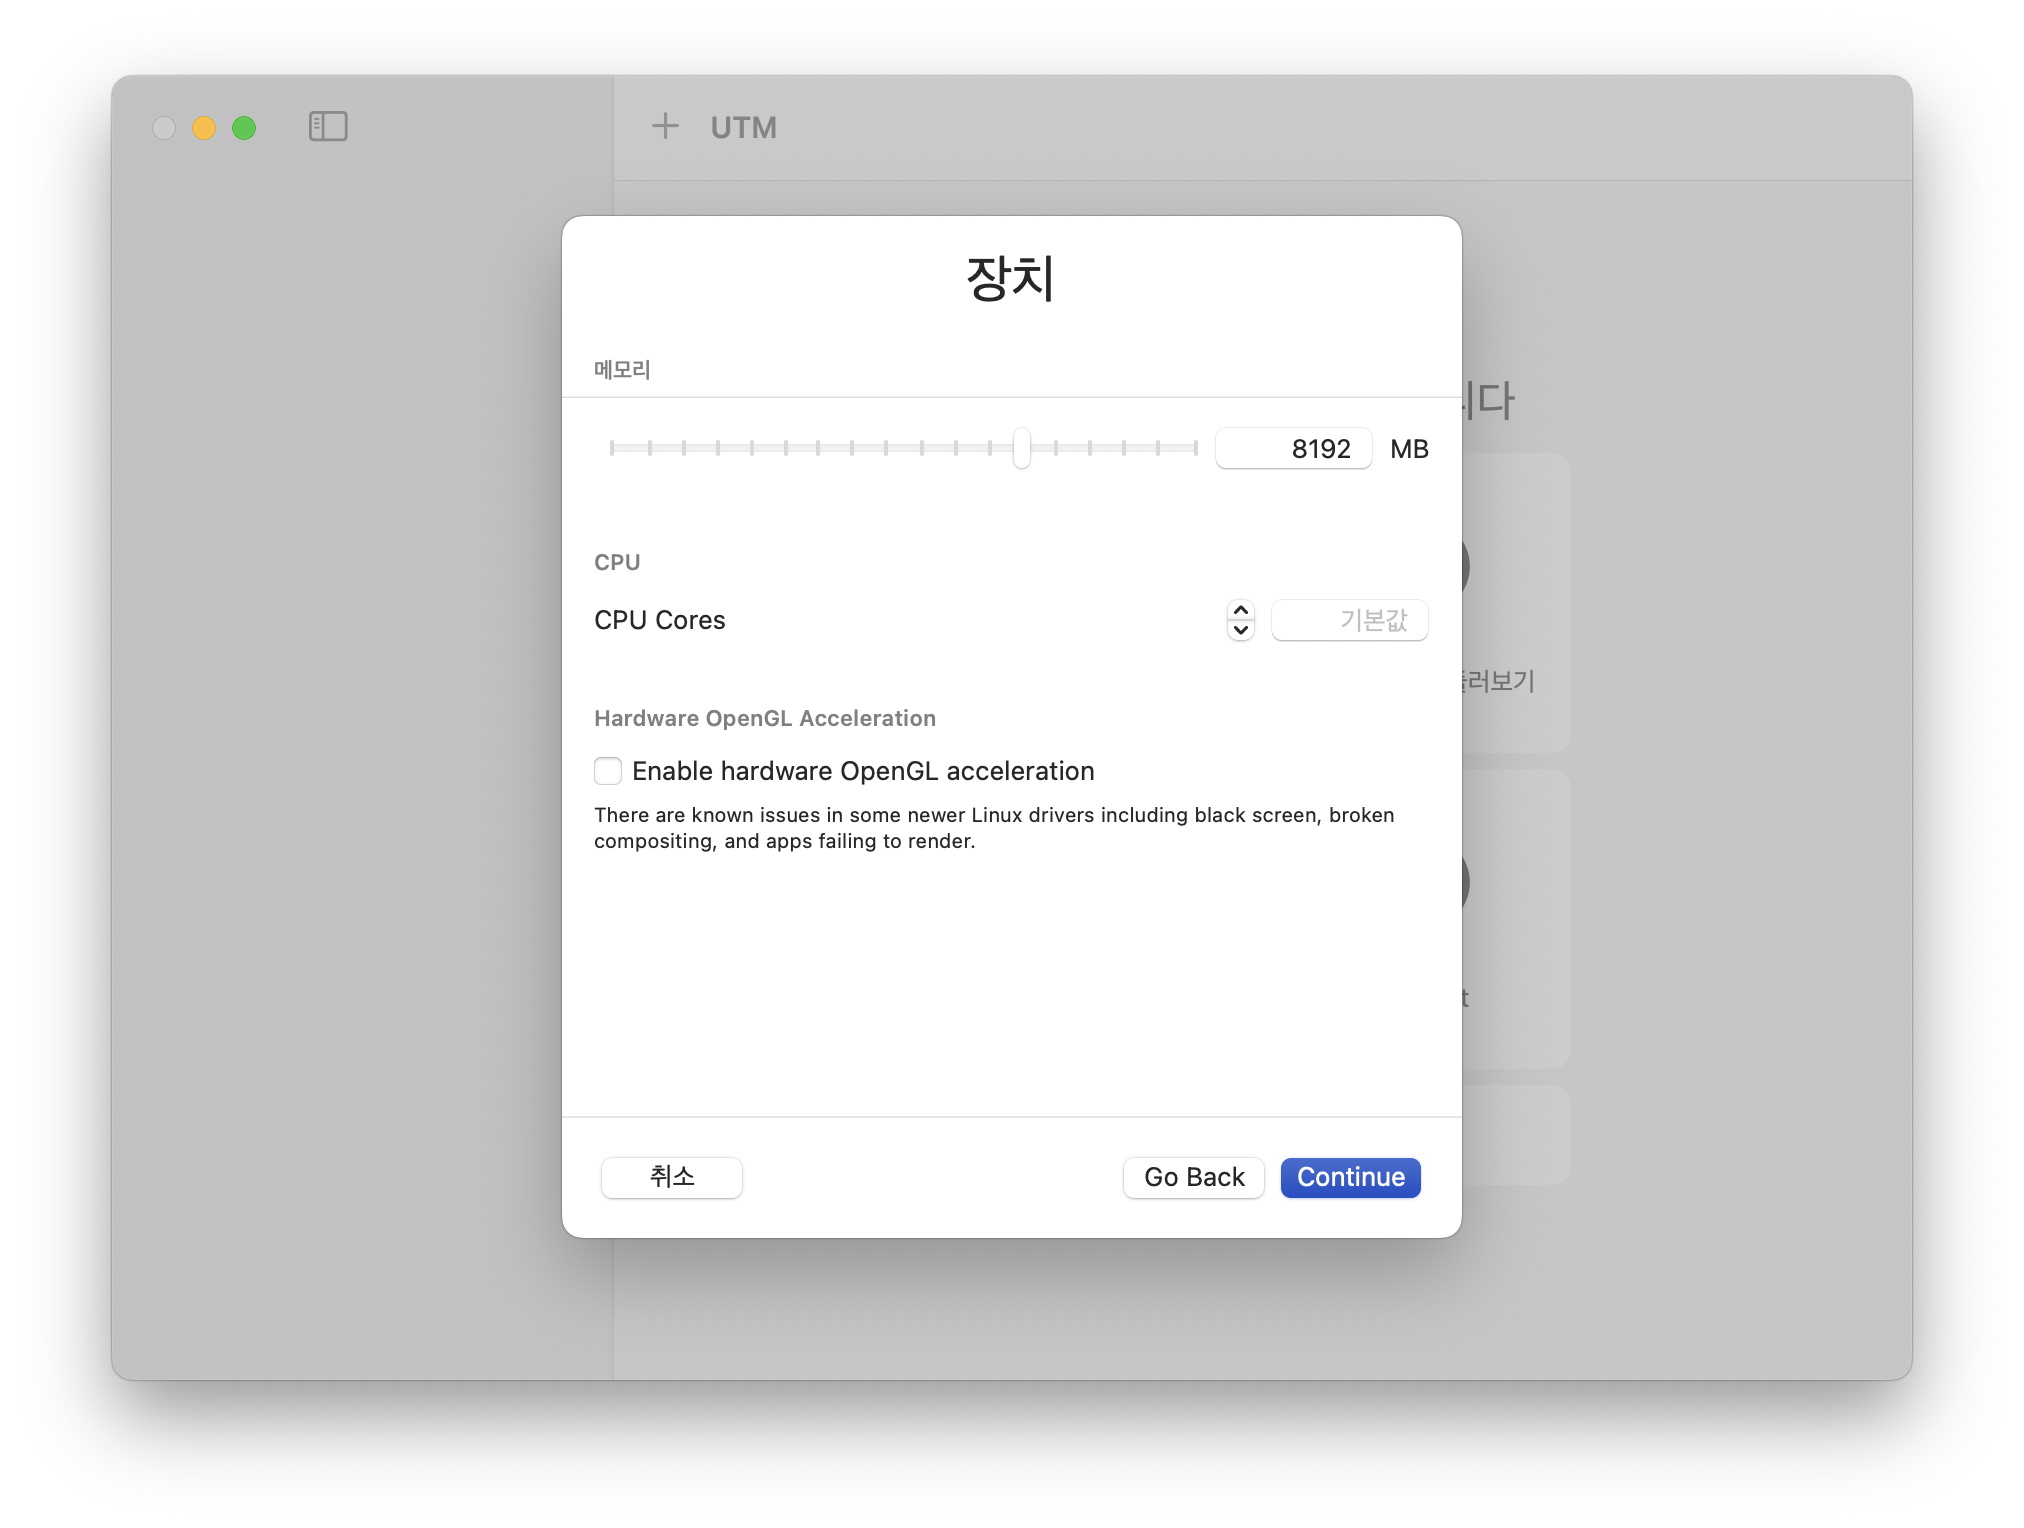
\includegraphics[width=0.9\textwidth]{images/chapter2Images/ch2_image_09.png}
    \caption{초기 Ubuntu 로그인 화면}
\end{figure}

\begin{figure}[htbp]
    \centering
    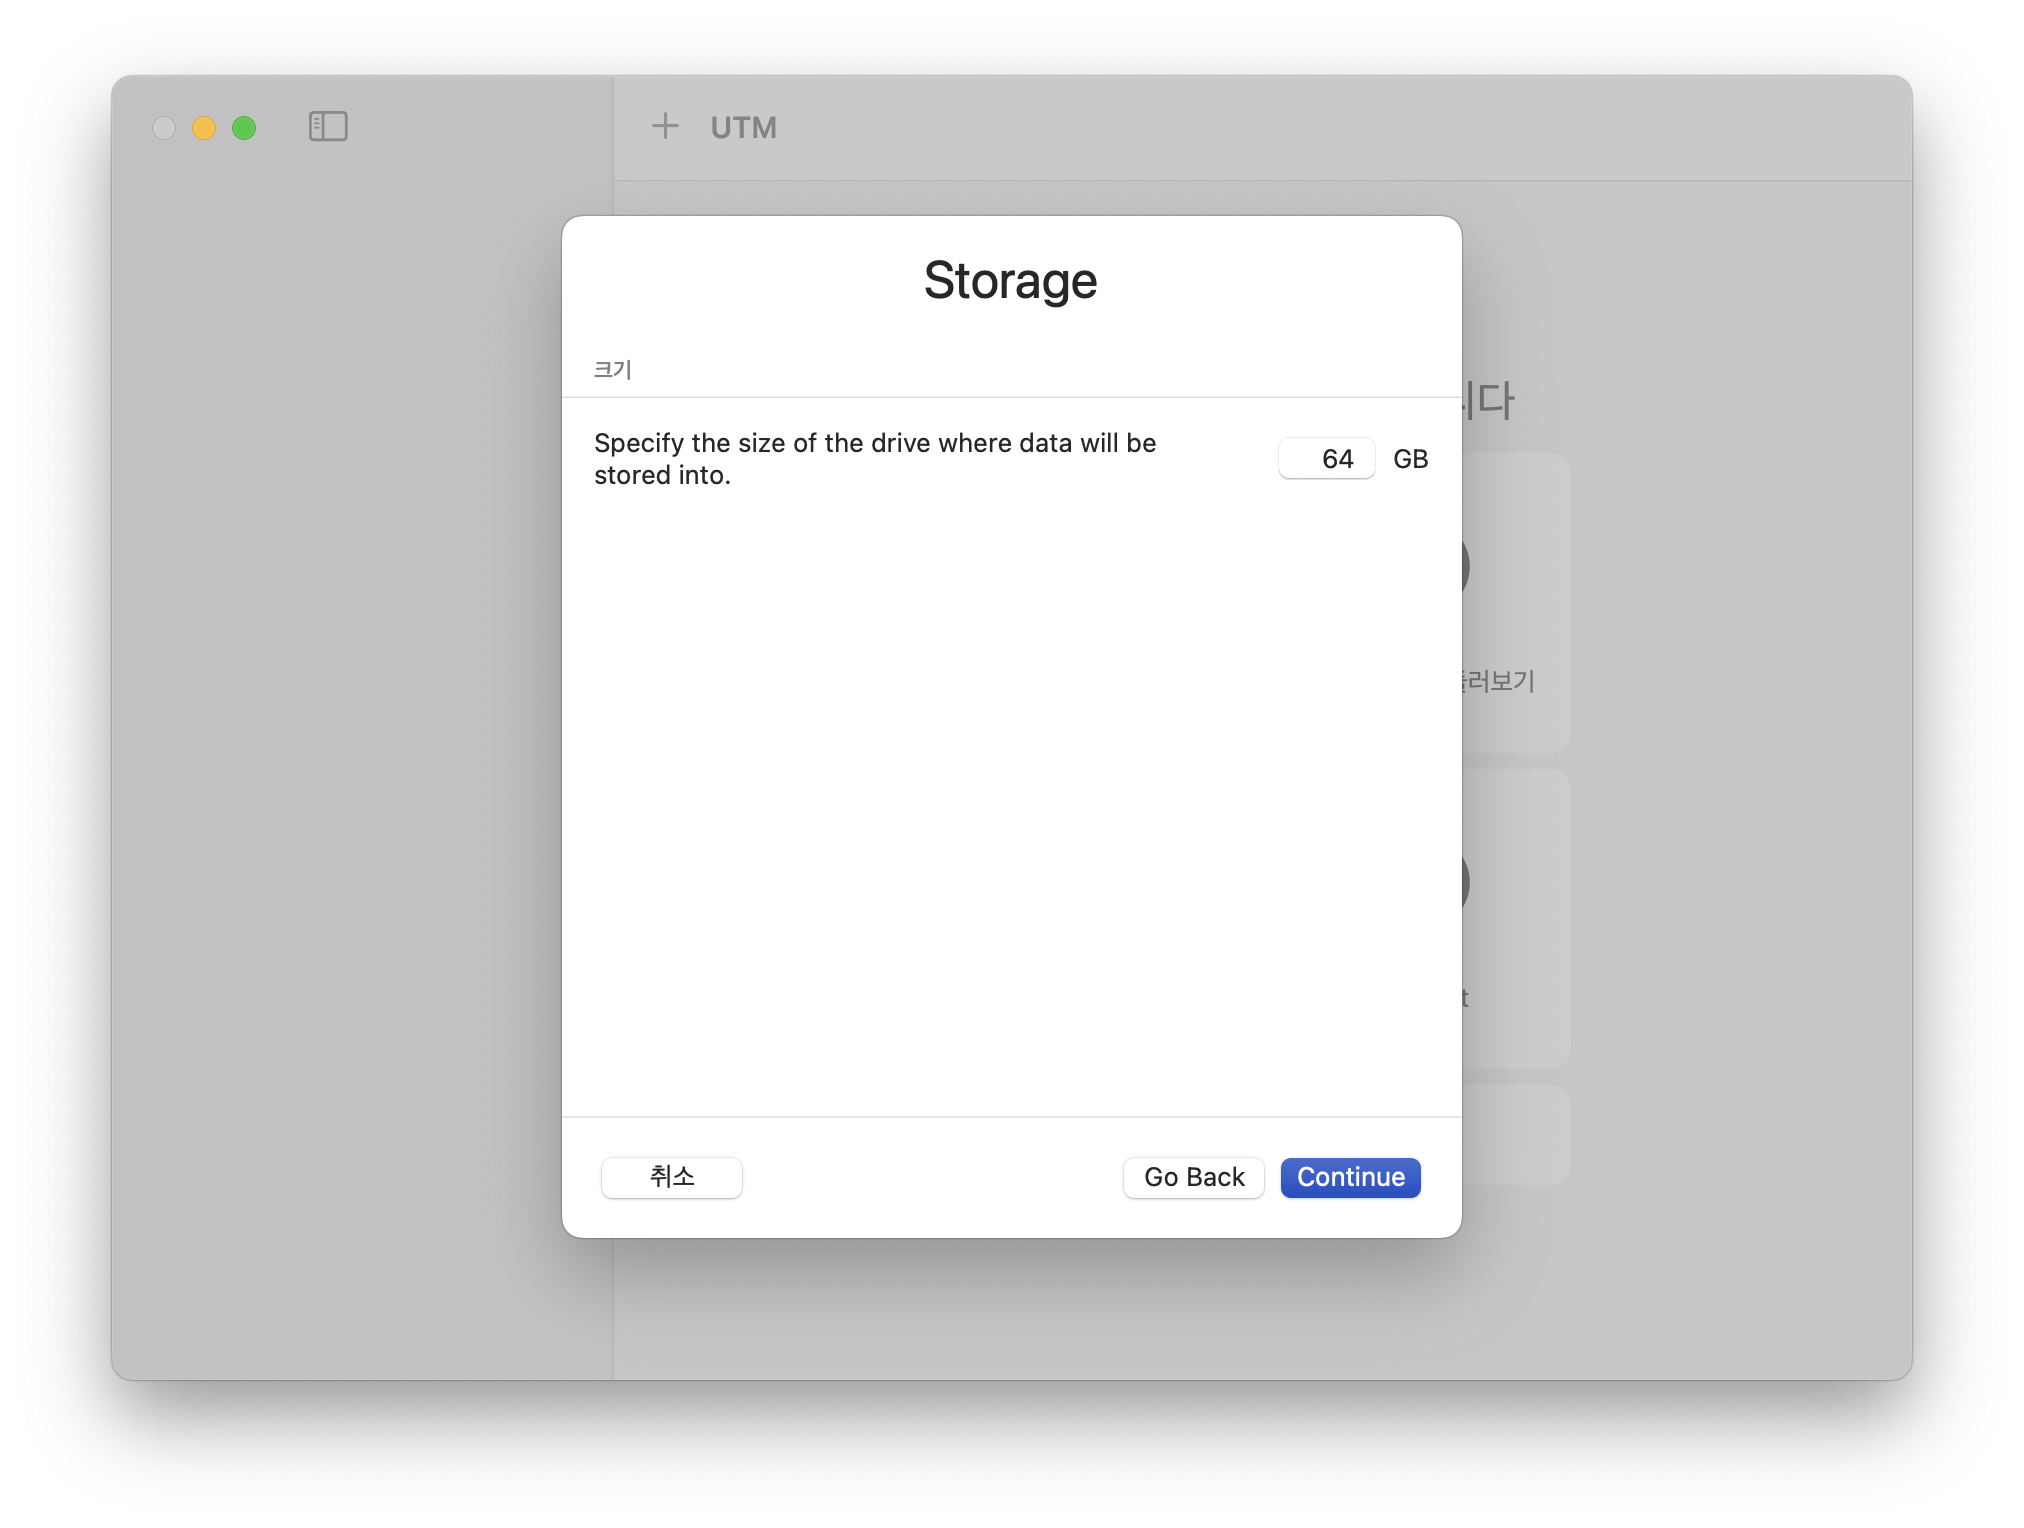
\includegraphics[width=0.9\textwidth]{images/chapter2Images/ch2_image_10.png}
    \caption{Ubuntu 데스크탑 환경}
\end{figure}

\begin{figure}[htbp]
    \centering
    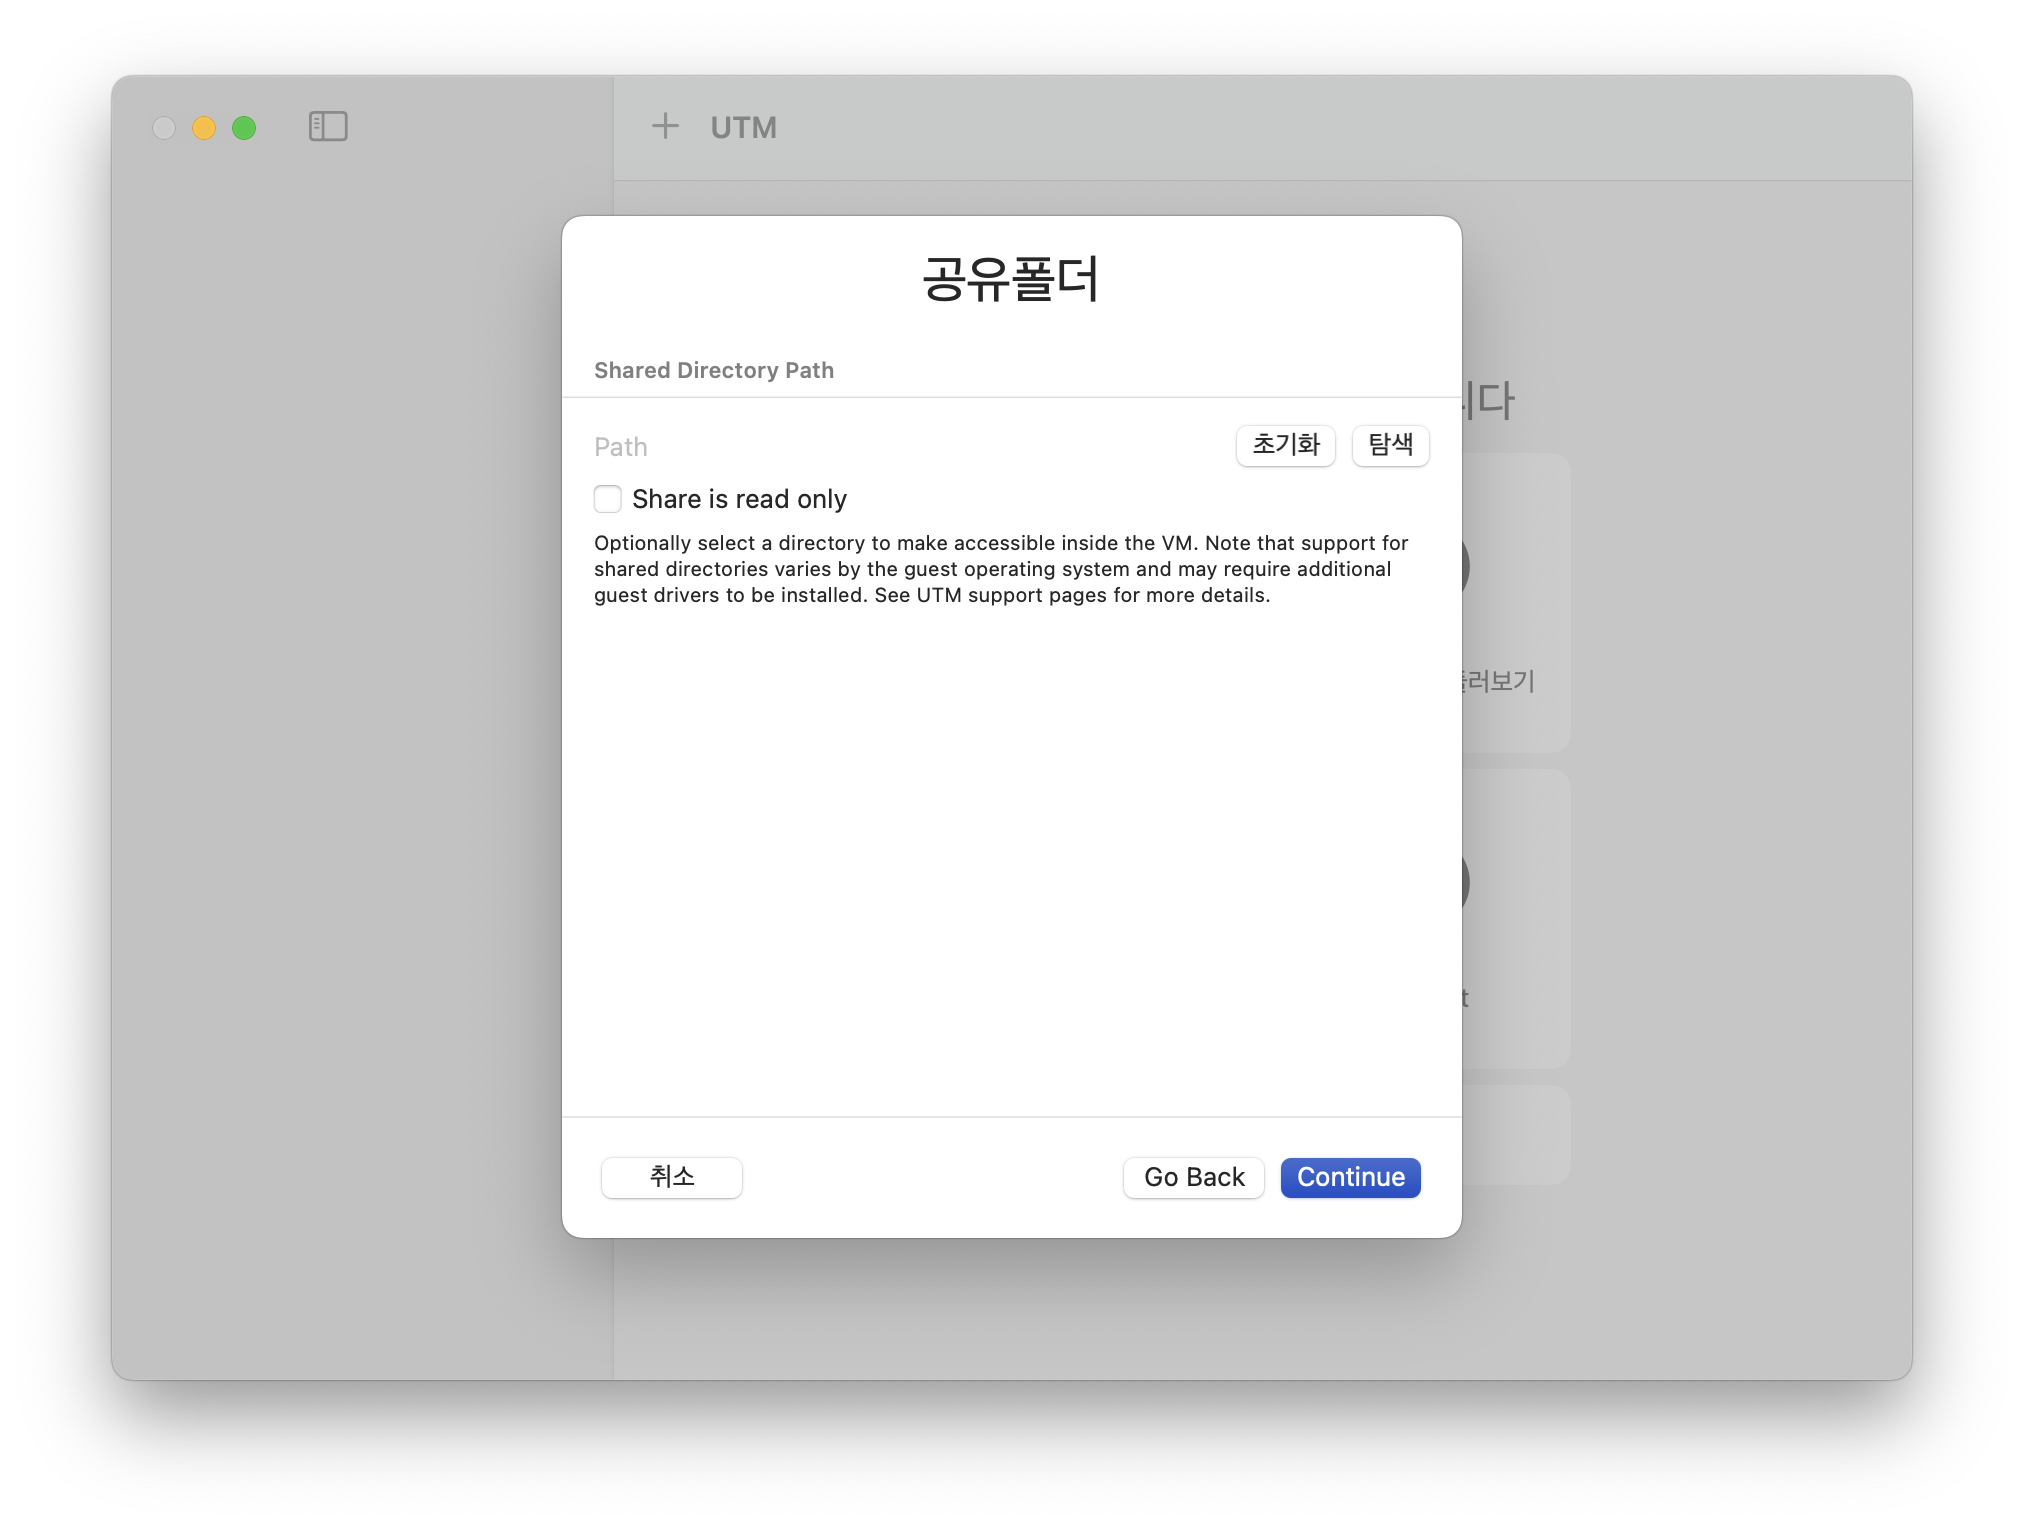
\includegraphics[width=0.9\textwidth]{images/chapter2Images/ch2_image_11.png}
    \caption{사용자 설정}
\end{figure}

\begin{figure}[htbp]
    \centering
    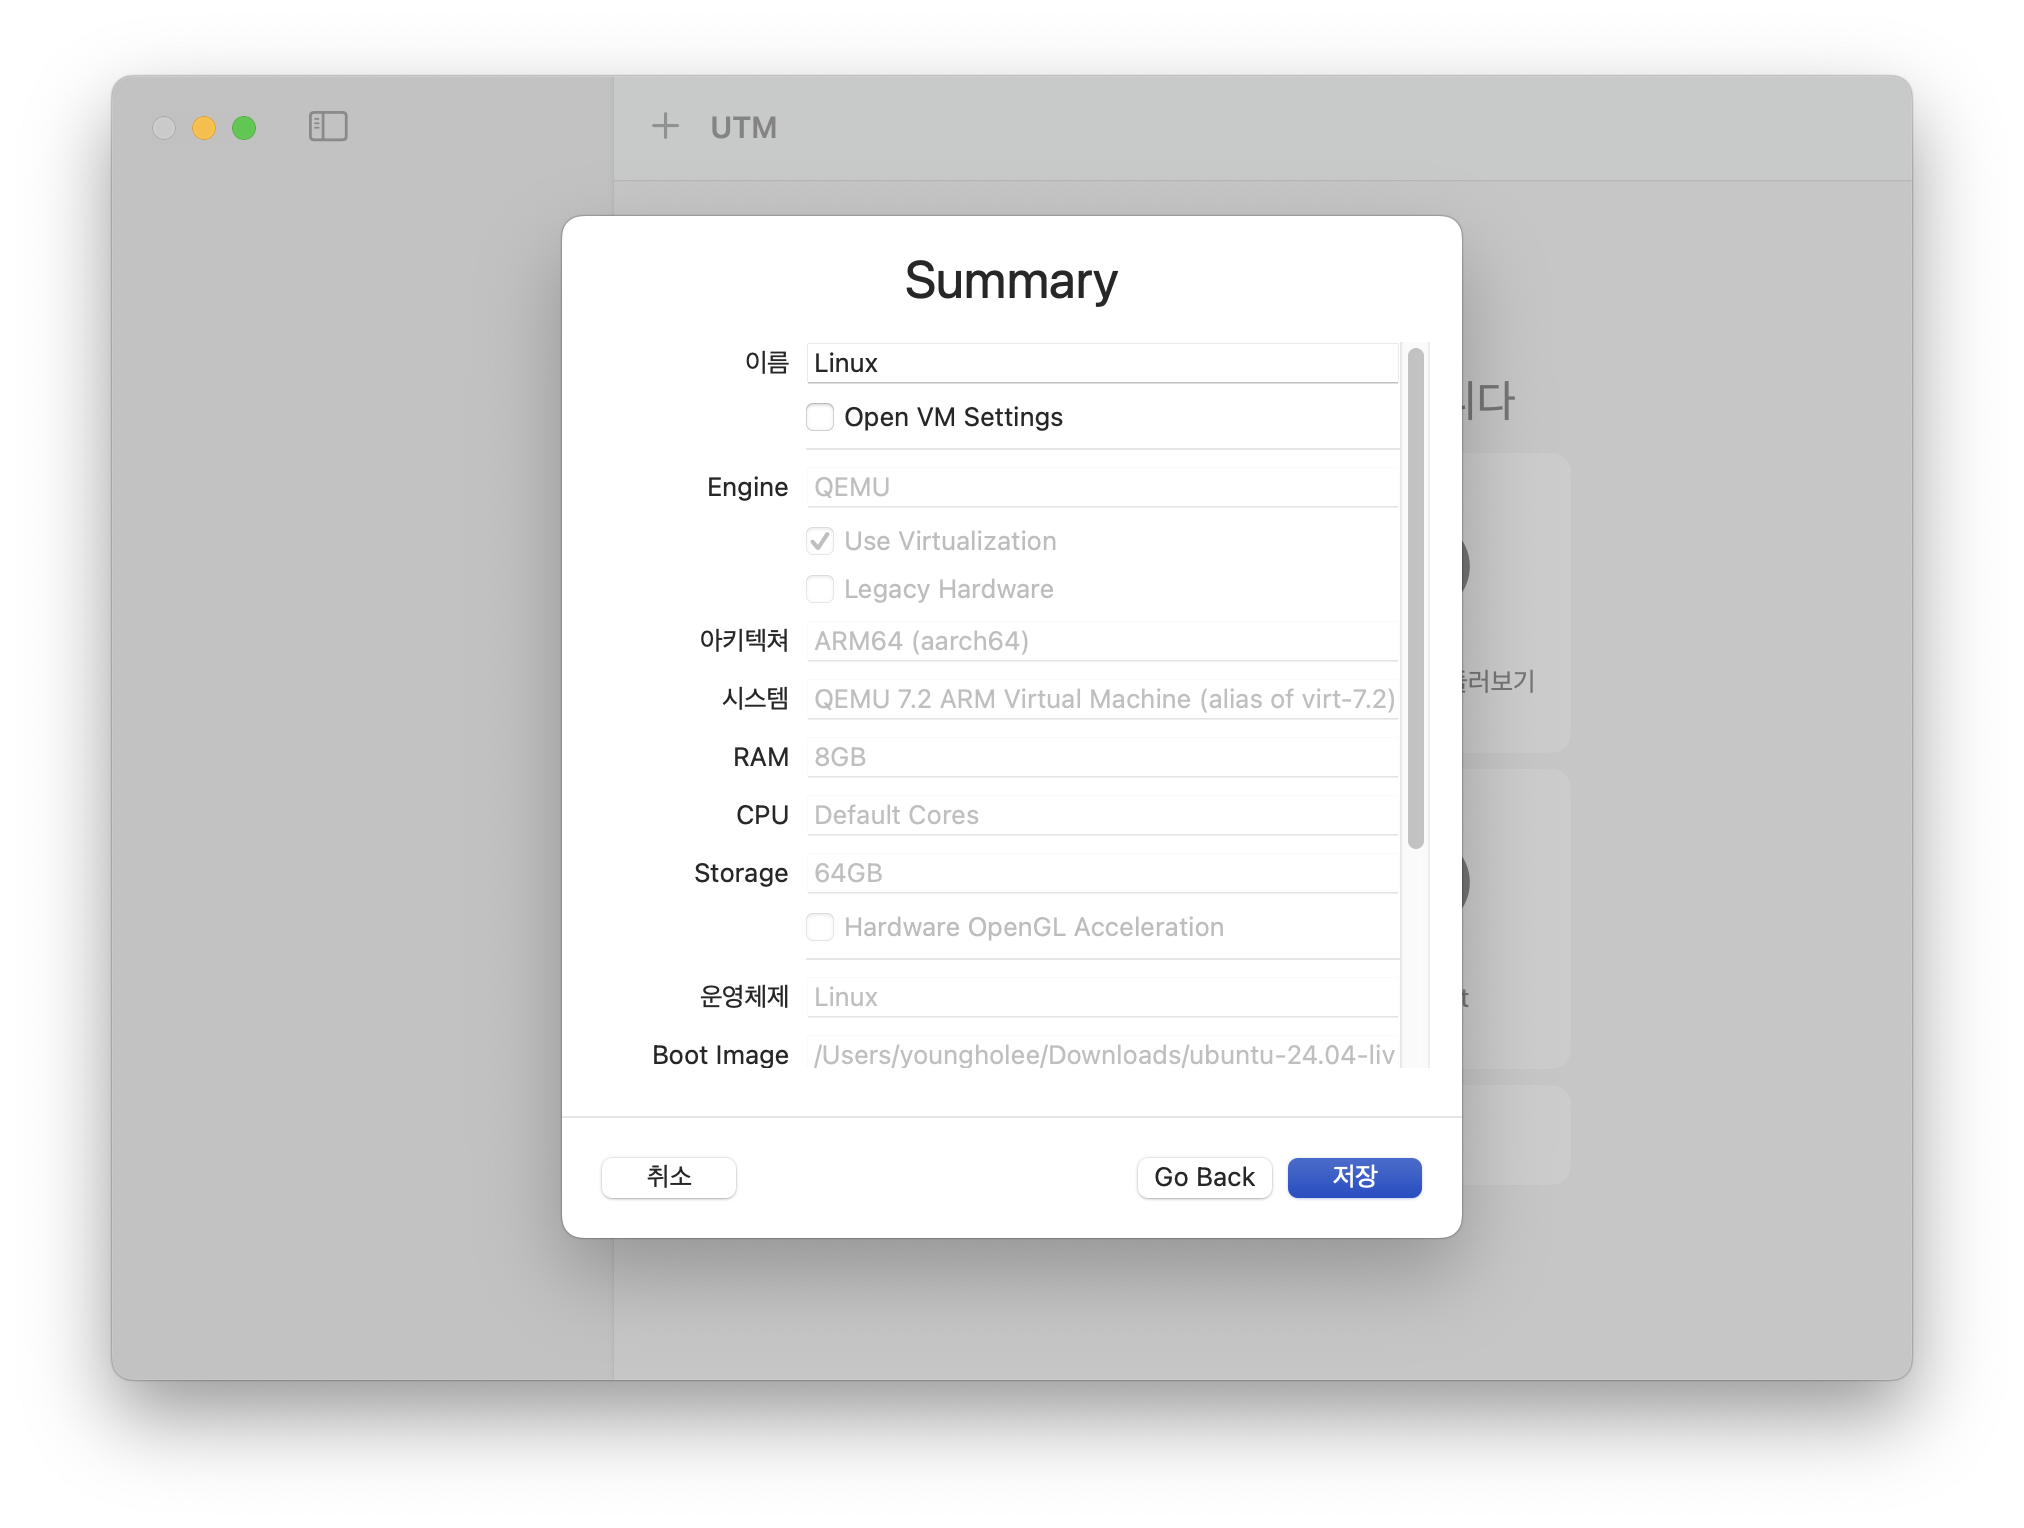
\includegraphics[width=0.9\textwidth]{images/chapter2Images/ch2_image_12.png}
    \caption{업데이트 설치}
\end{figure}

\begin{figure}[htbp]
    \centering
    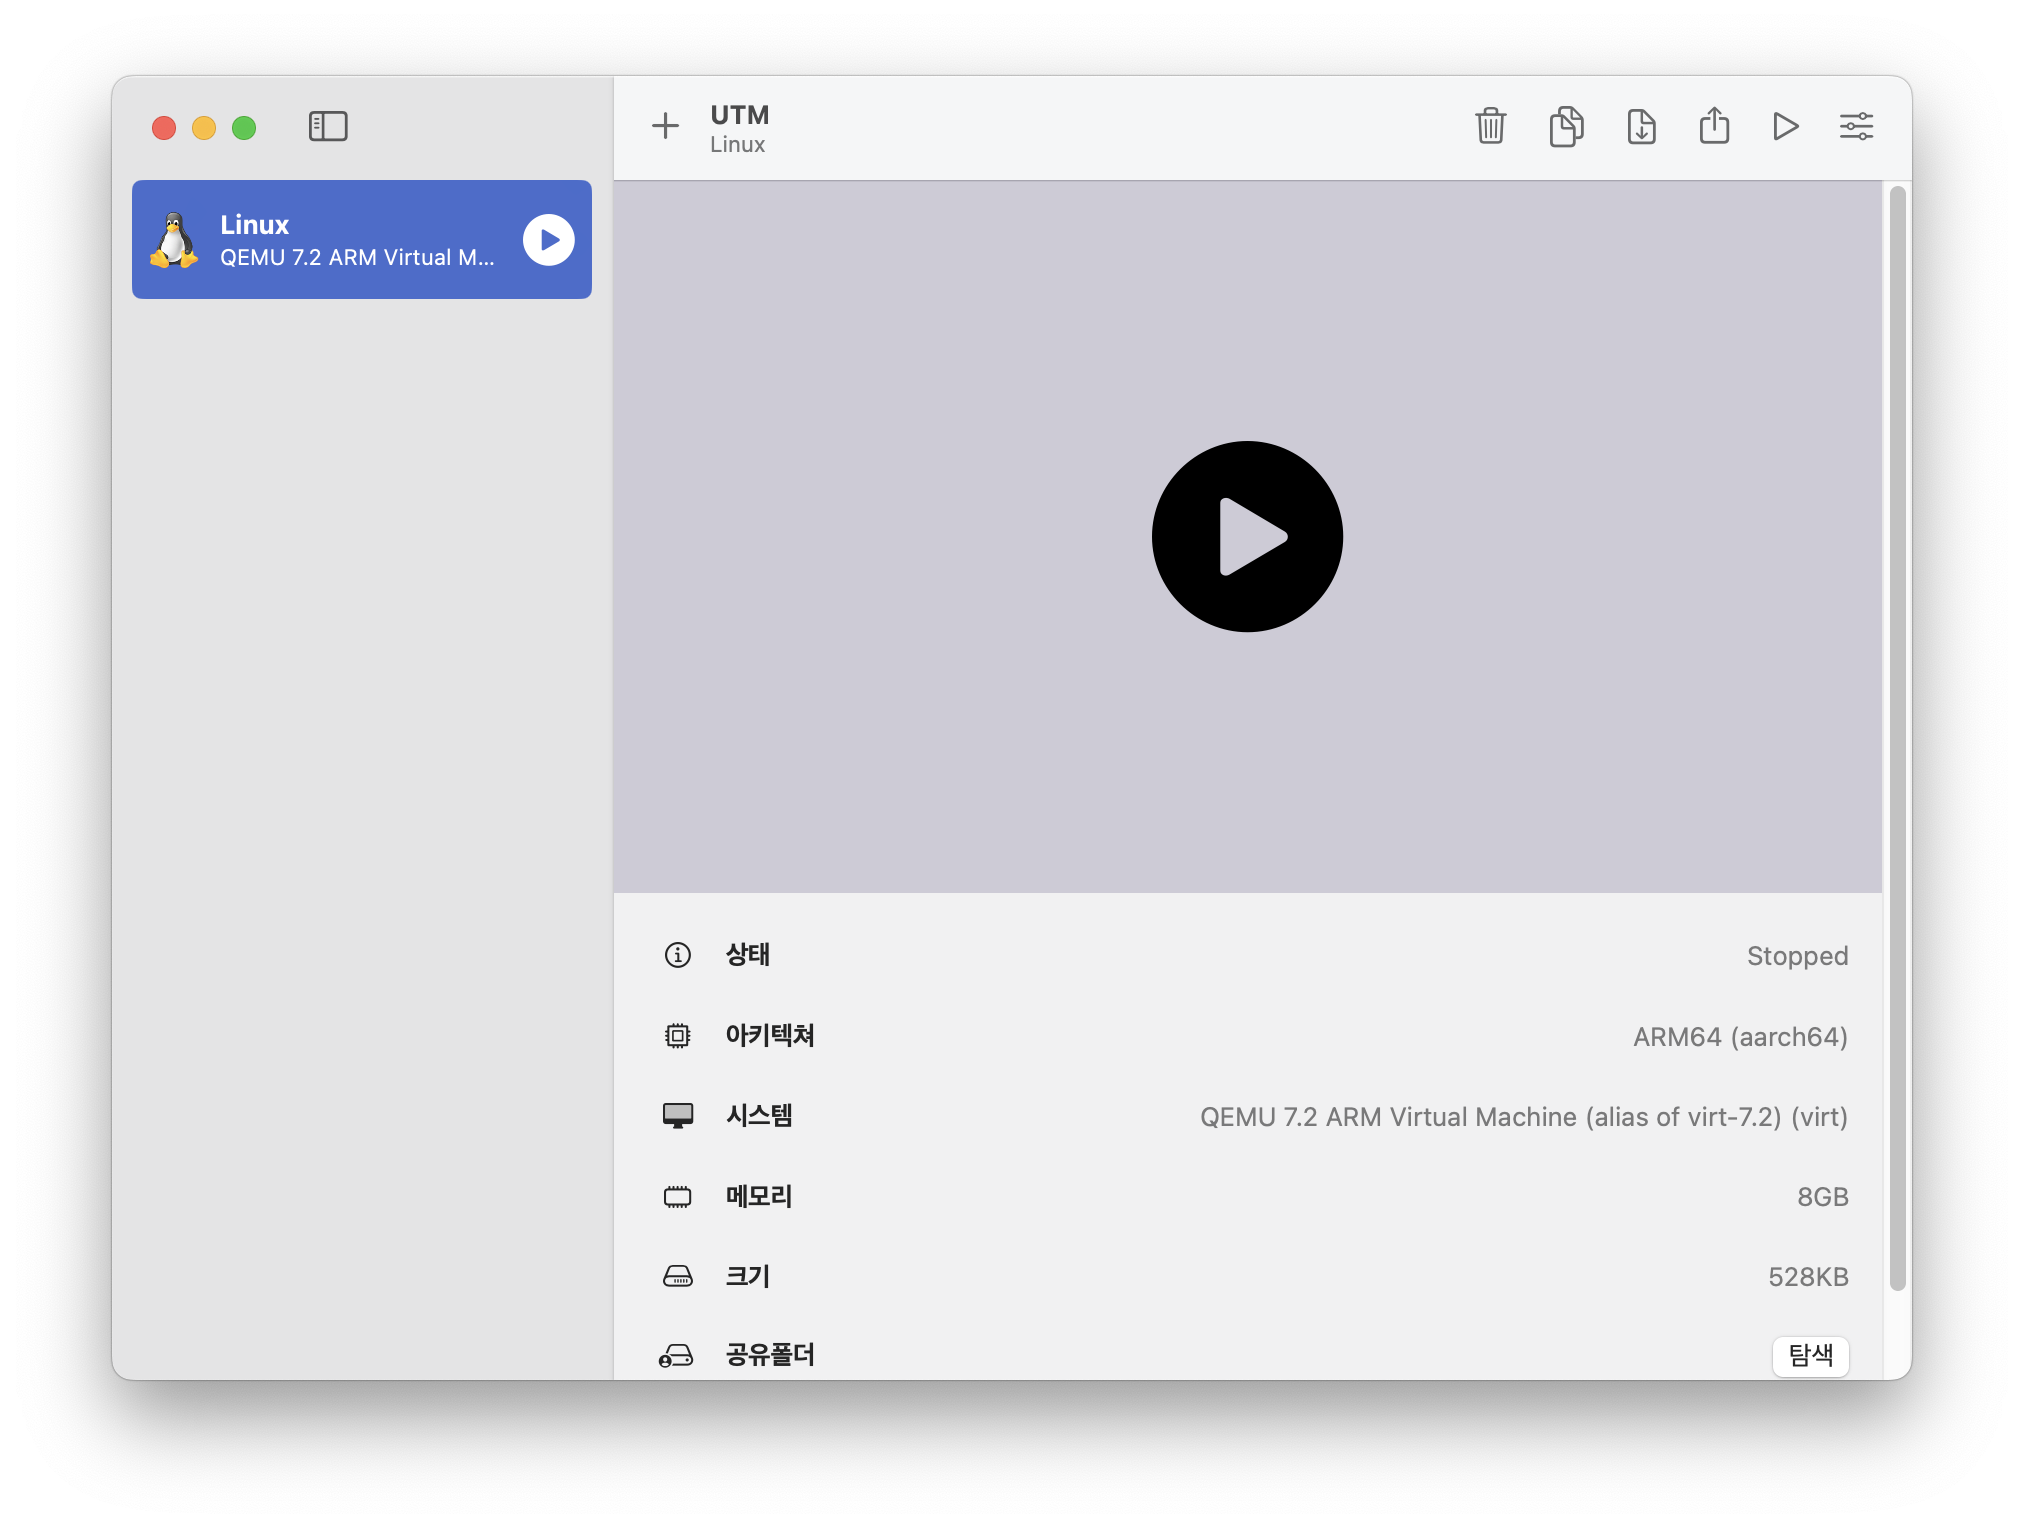
\includegraphics[width=0.9\textwidth]{images/chapter2Images/ch2_image_13.png}
    \caption{시스템 사용 준비 완료}
\end{figure}

\begin{figure}[htbp]
    \centering
    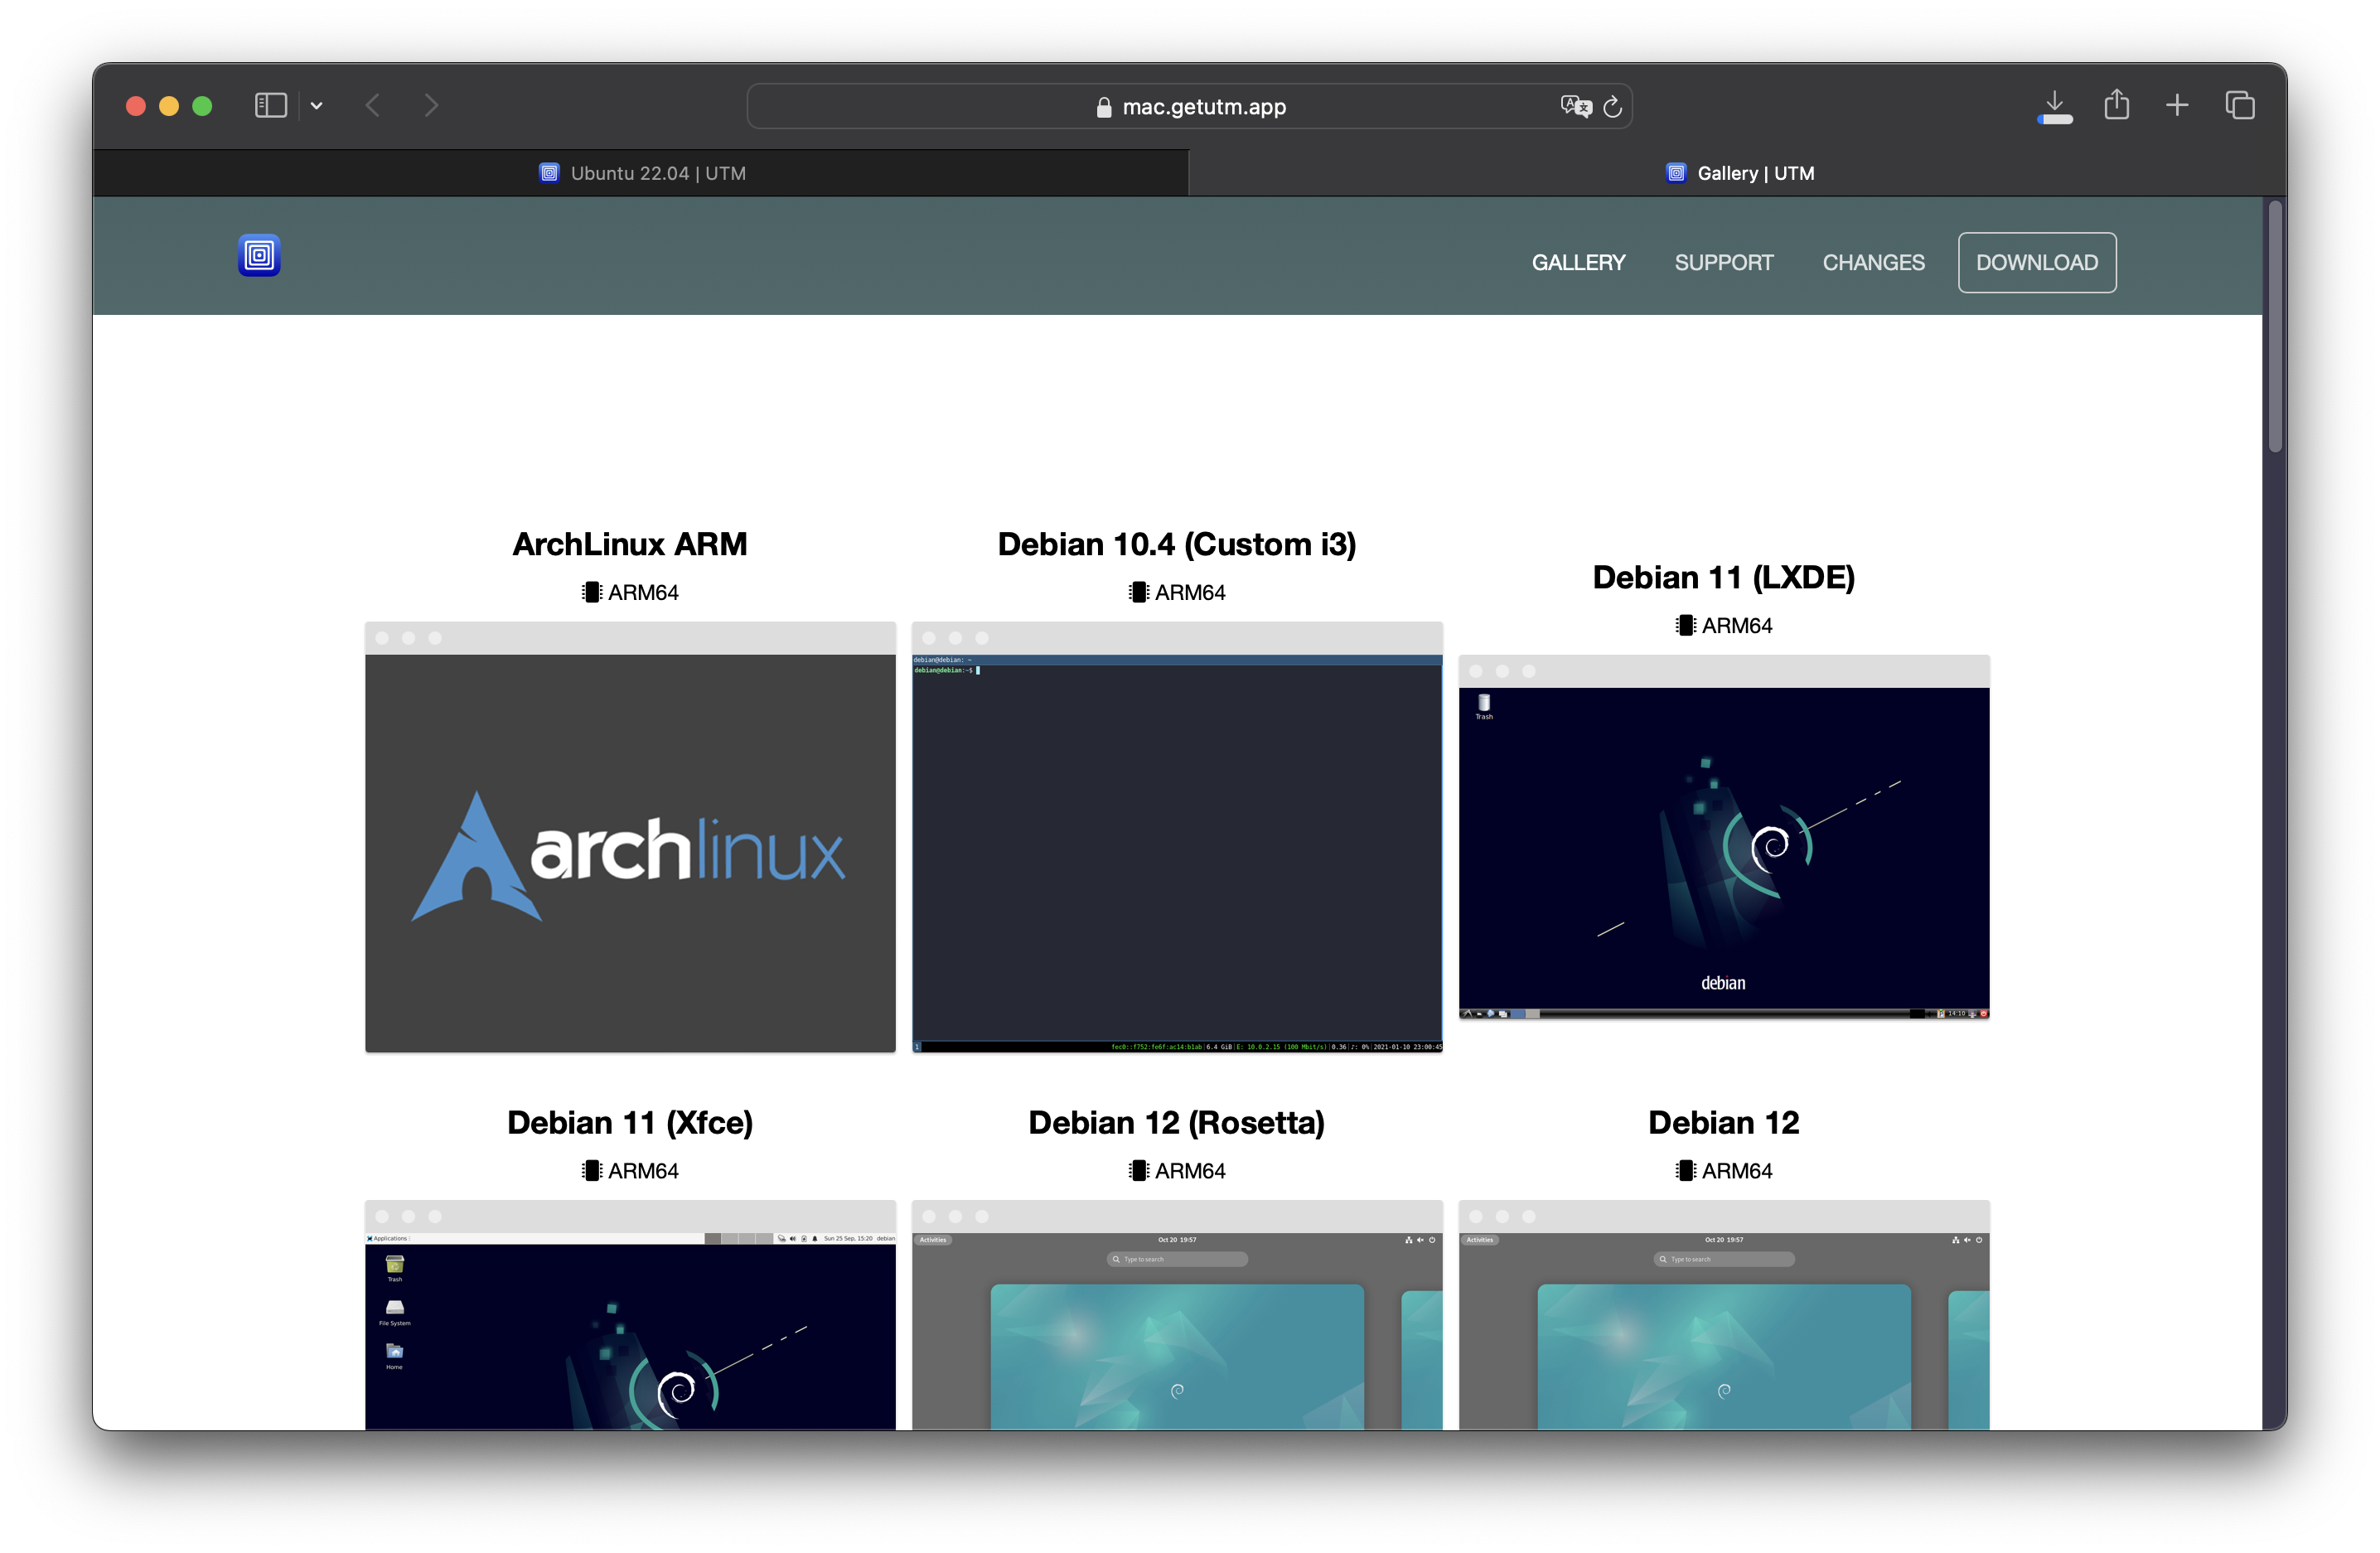
\includegraphics[width=0.9\textwidth]{images/chapter2Images/ch2_image_14.png}
    \caption{첫 번째 응용 프로그램 실행}
\end{figure}

\begin{figure}[htbp]
    \centering
    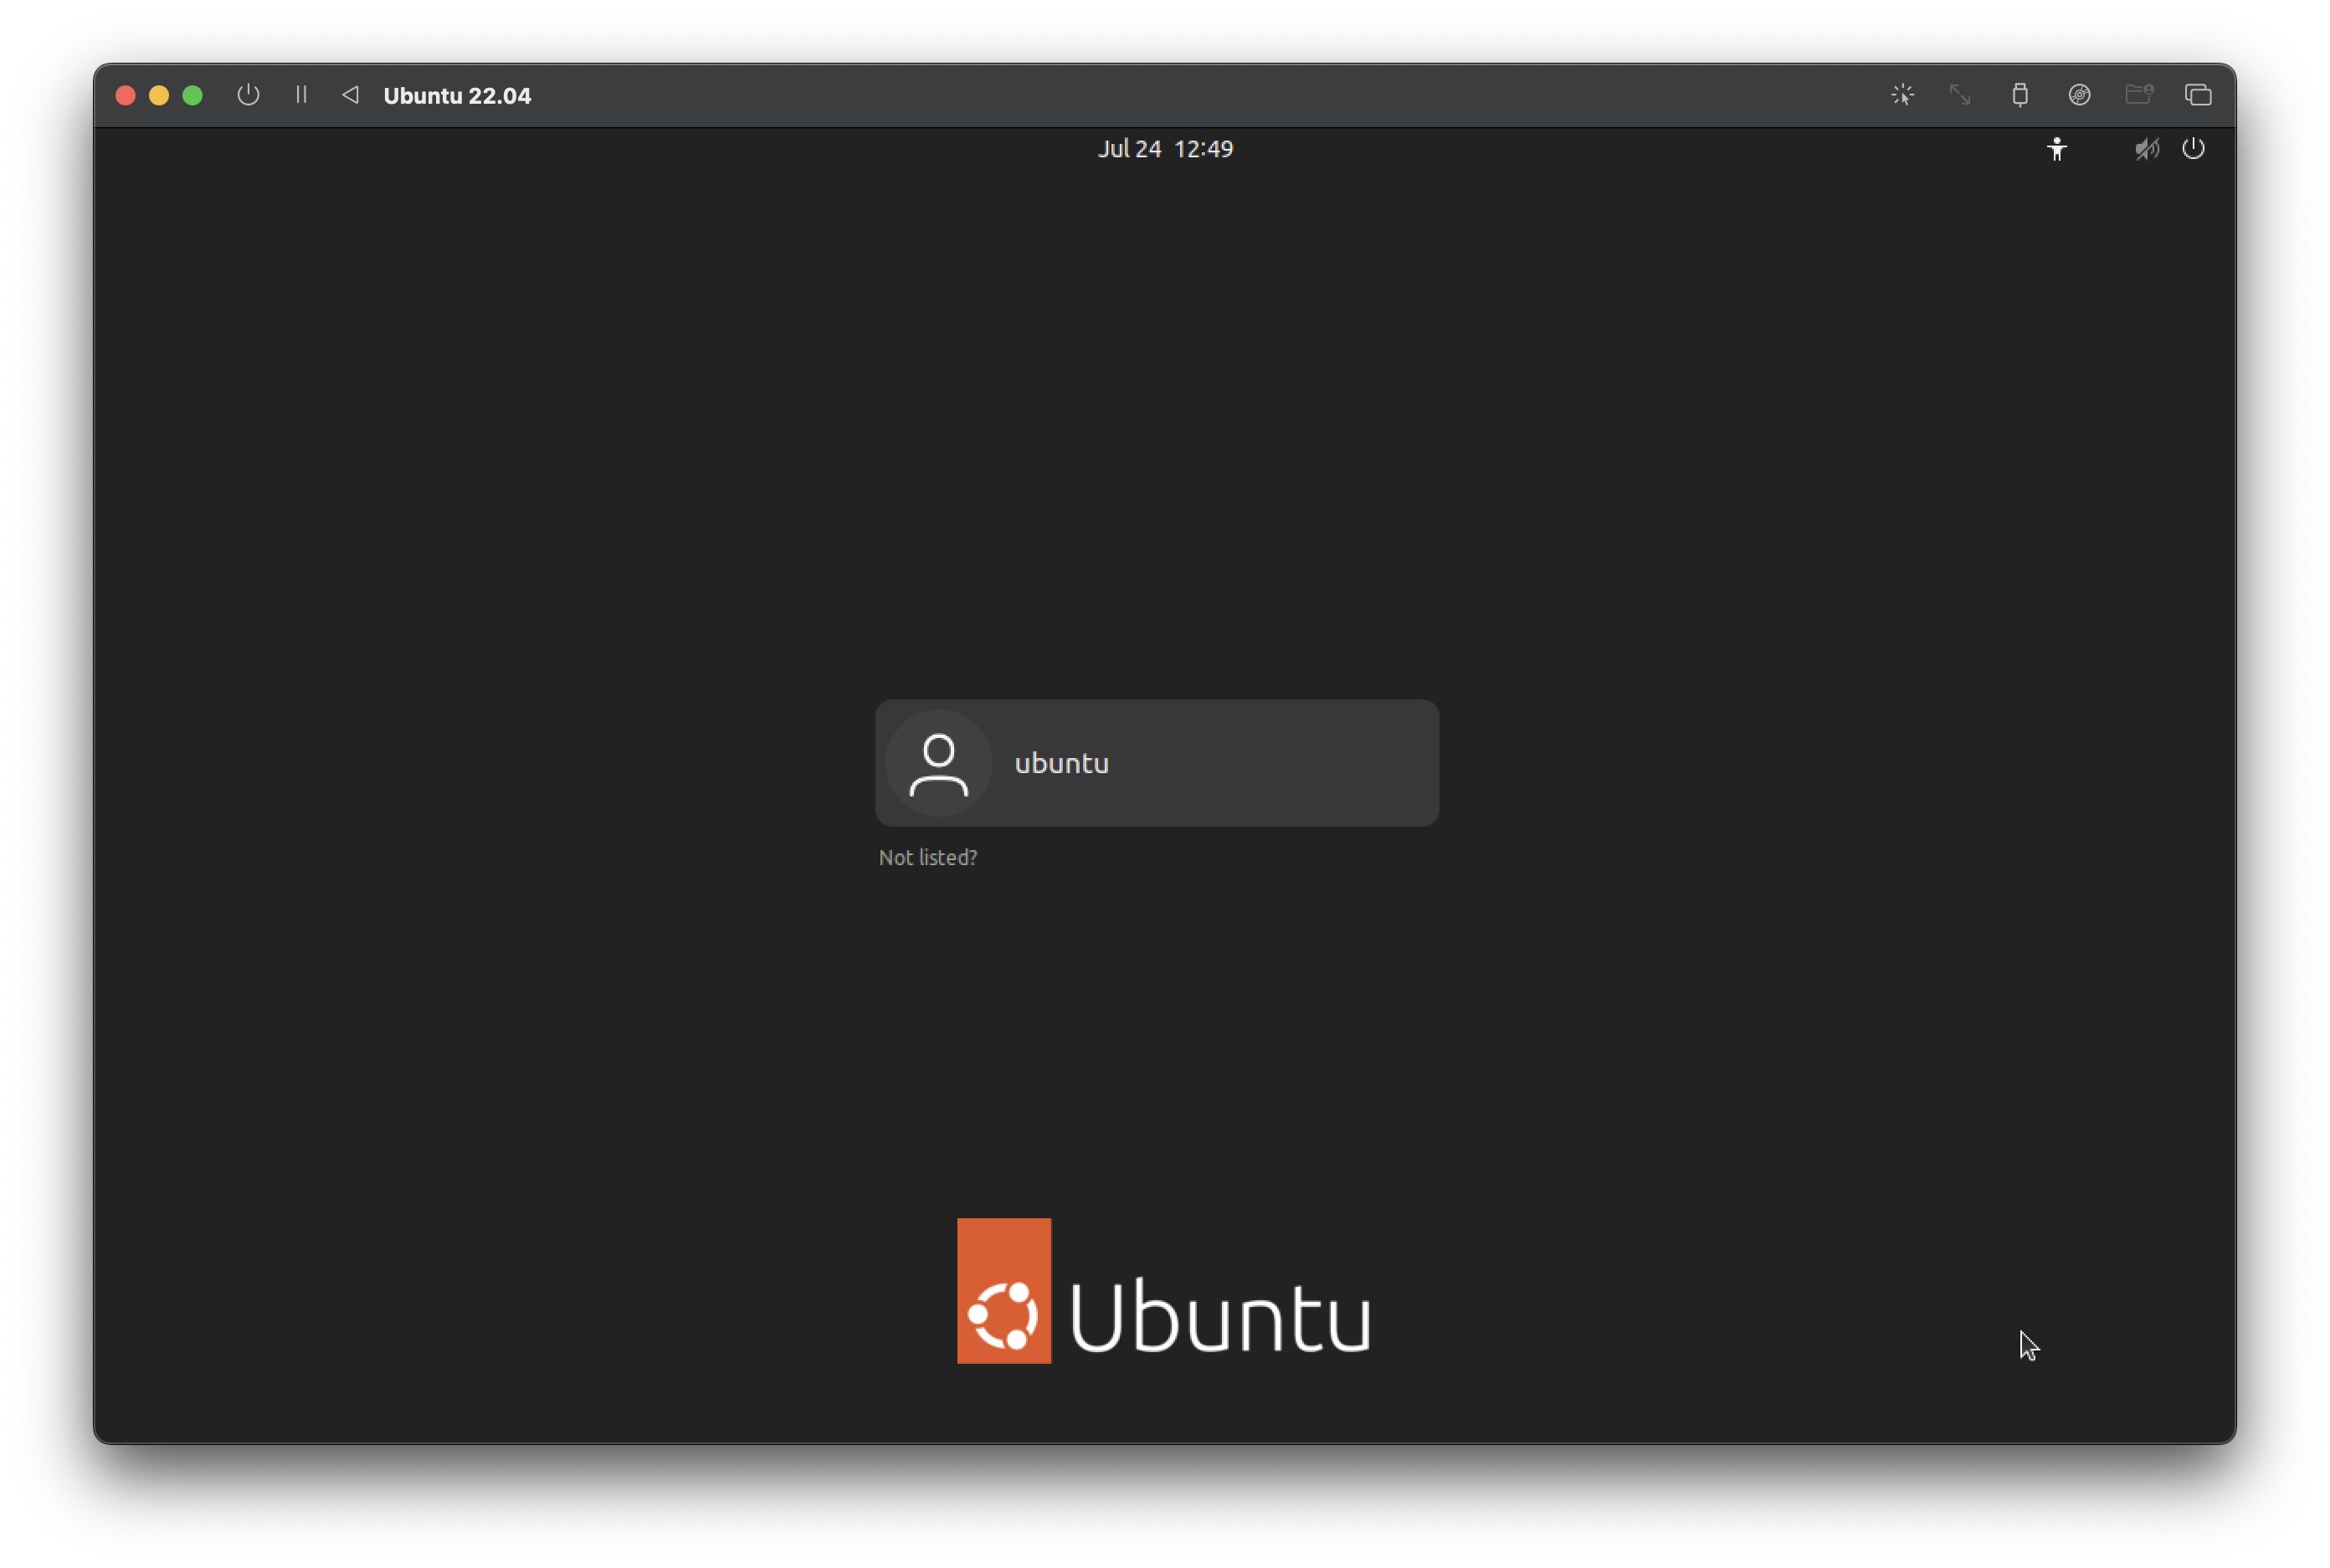
\includegraphics[width=0.9\textwidth]{images/chapter2Images/ch2_image_15.png}
    \caption{Ubuntu 기능 탐색}
\end{figure}

\begin{figure}[htbp]
    \centering
    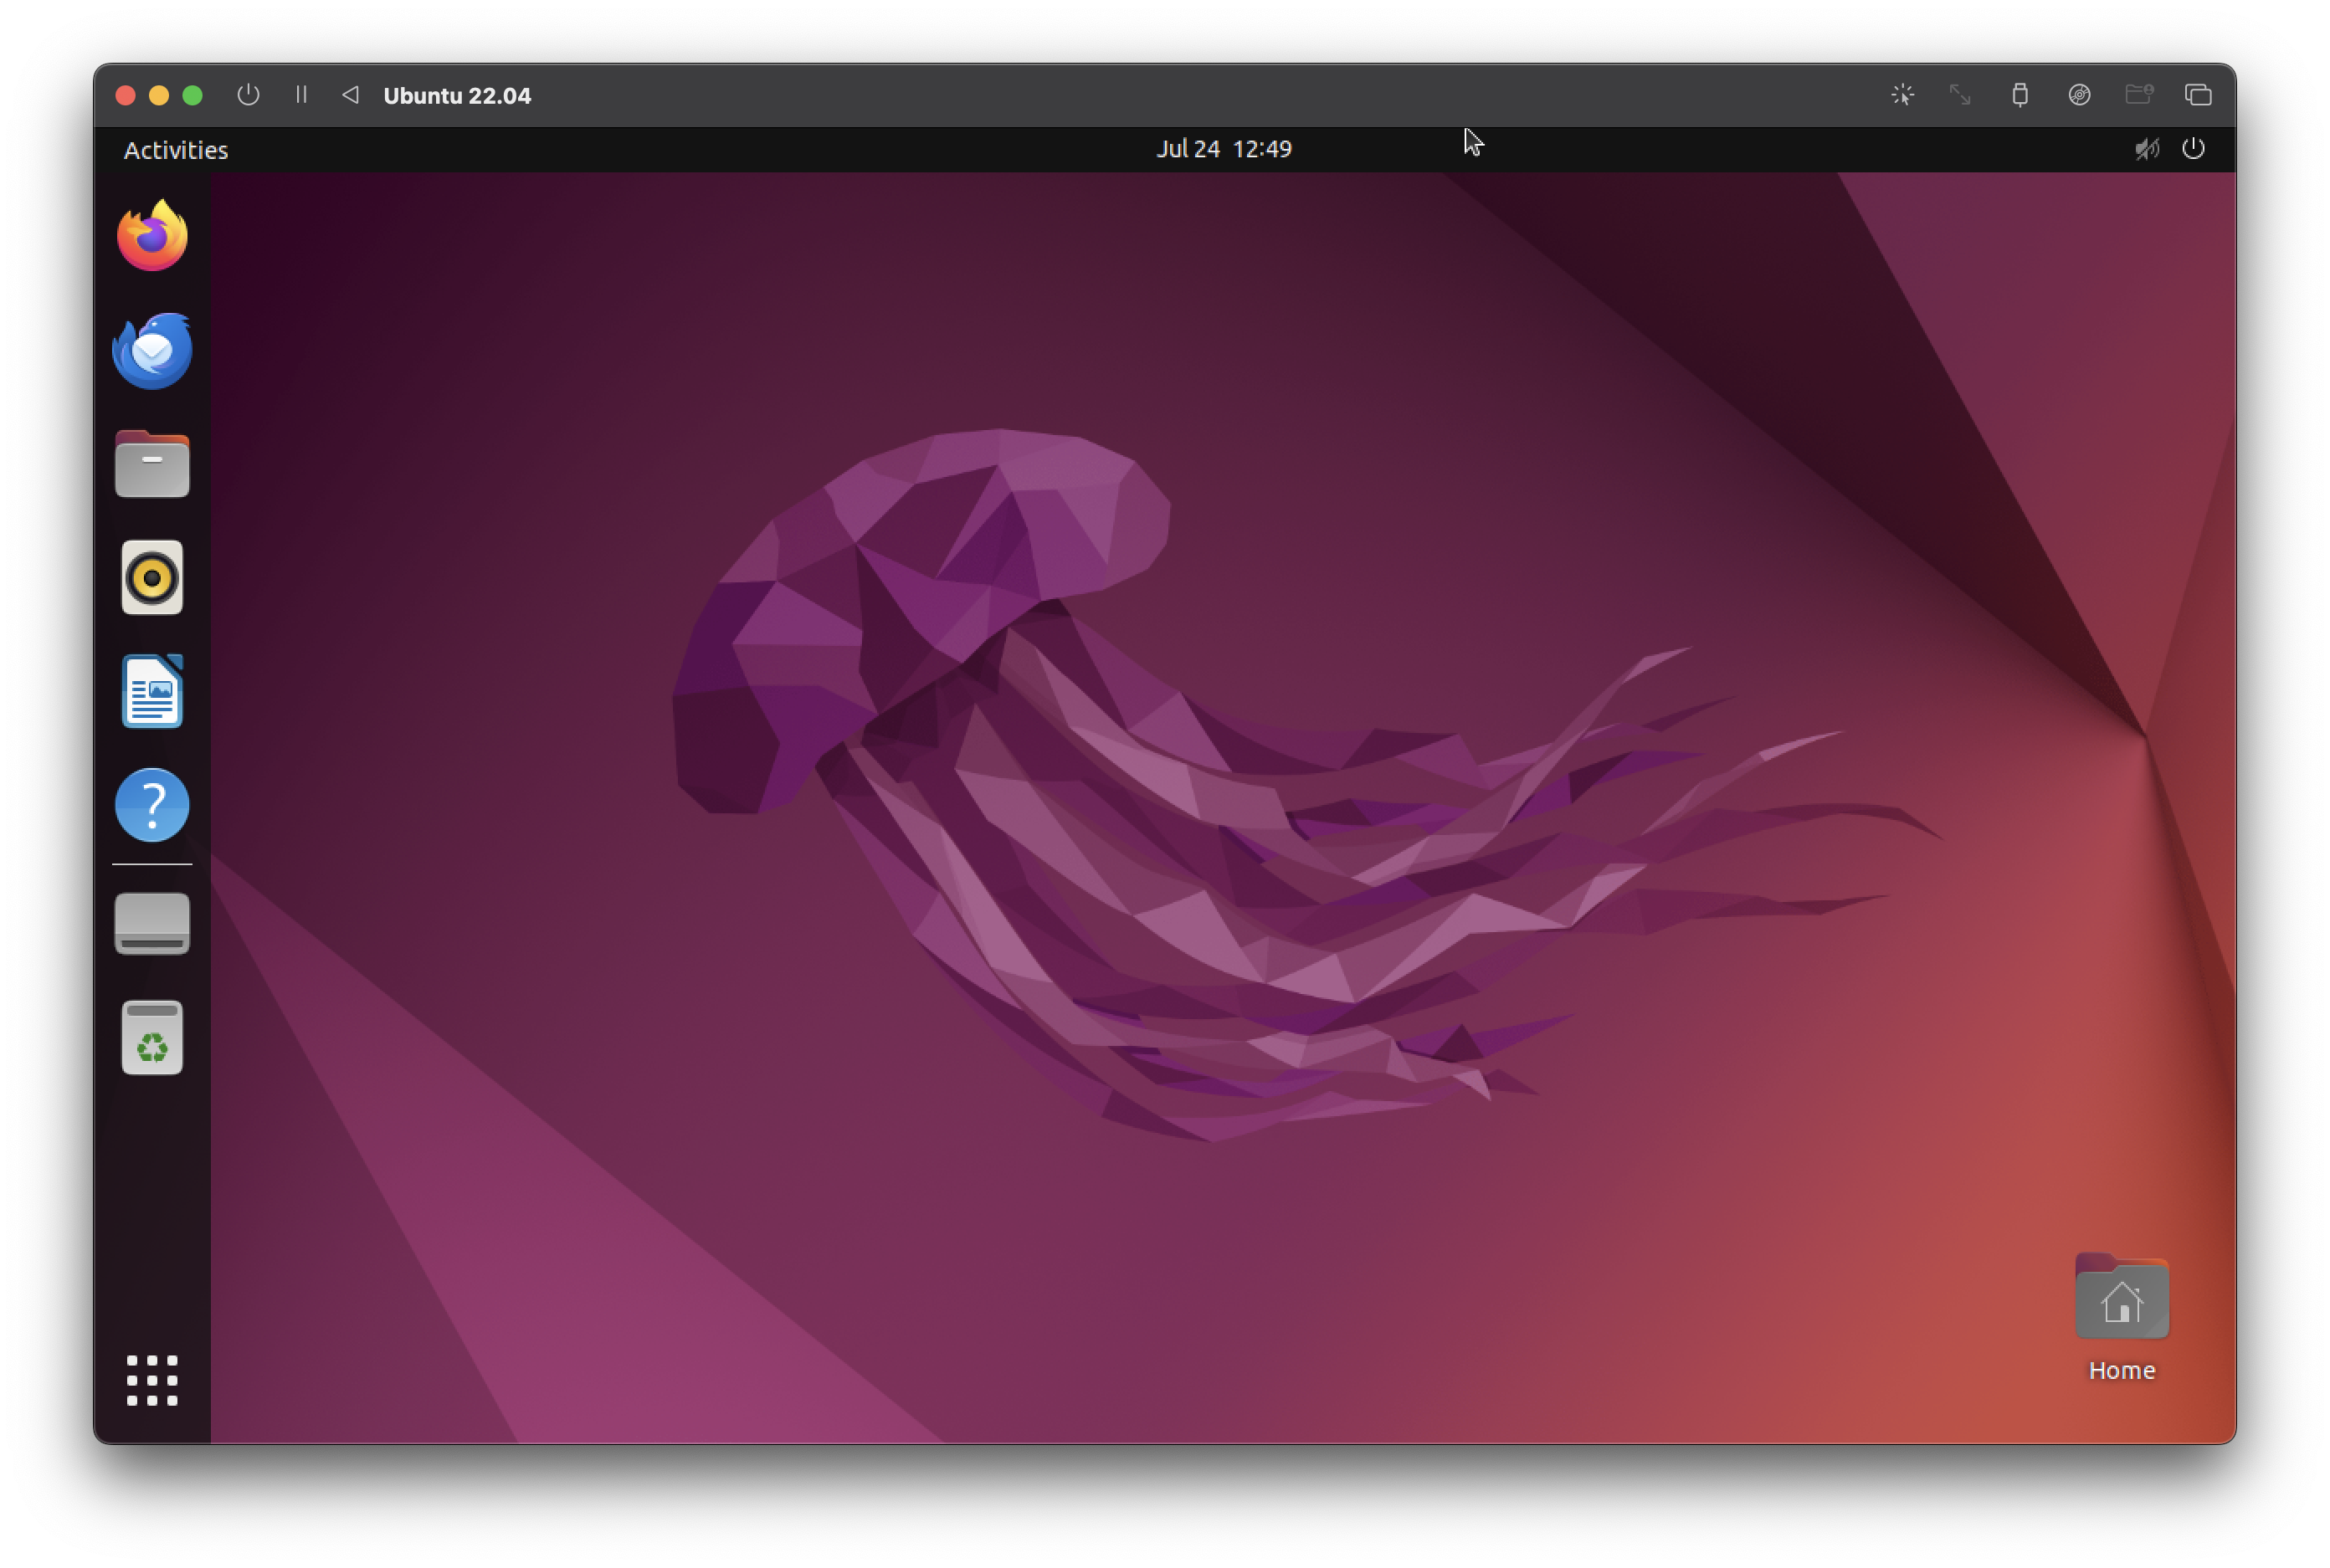
\includegraphics[width=0.9\textwidth]{images/chapter2Images/ch2_image_16.png}
    \caption{Ubuntu 완전 작동}
\end{figure}